% The contents of this file is 
% Copyright (c) 2009-  Charles R. Severance, All Righs Reserved

%\chapter{Using databases and Structured Query Language (SQL)}
\chapter{Banco de Dados e Structured Query Language (SQL)}

%\section{What is a database?}
\section{O que é um banco de dados?}
\index{database}

%A {\bf database} is a file that is organized for storing data.
%Most databases are organized like a dictionary in the sense
%that they map from keys to values.  The biggest difference
%is that the database is on disk (or other permanent storage),
%so it persists after the program ends.  Because a database is
%stored on permanent storage, it can store far more data than
%a dictionary, which is limited to the size of the memory 
%in the computer.

Um {\bf banco de dados} é um tipo de arquivo organizado para armazenamento de
dados. A maioria dos bancos de dados são orgazanizados como um dicionário, no
sentido de que eles realizam o mapeamento por chaves e valores. A grande
diferença é que os bancos de dados estão em disco (ou outros dispositivos de
armazenamentos permanentes), então eles continuam armazenando os dados mesmo
depois que o programa termina. Porque um banco de dados é armazenado de forma
permanente, isto permite armazenar muito mais dados que um dicionário, que é
limitado ao tamanho da memória no computador.

\index{database!indexes}
%Like a dictionary, database software is designed to keep 
%the inserting and accessing of data very fast, even for large
%amounts of data.   Database software maintains its performance by 
%building {\bf indexes} as data is added to the database
%to allow the computer to jump quickly to a particular
%entry.

Como um dicionário, um banco de dados é um software desenvolvido para manter a
inserção e acesso aos dados de forma muito rápida, até para grandes volumes de
dados. O banco de dados mantém sua performance através da construção de
{\bf indices} assim que o dado é adicionado, isto permite ao computador acessar
rapidamente uma entrada em particular.

%There are many different database systems which are used for a wide
%variety of purposes including: Oracle, MySQL, Microsoft SQL Server, 
%PostgreSQL, and SQLite.  We focus on SQLite in this book because
%it is a very common database and is already built into Python.  
%SQLite is designed to be \emph{embedded} into other applications
%to provide database support within the application.  For example,
%the Firefox browser also uses the SQLite database internally as do 
%many other products.

Existem diferentes tipos de sistemas de bancos de dados que são utilizados 
para diferentes propósitos, alguns destes são: Oracle, MySQL, Microsoft SQL
Server, PostgreSQL, e SQLite. Focaremos no uso do SQLite neste livro pois é
um banco de dados comum e já está integrado ao Python. O SQLite foi
desenvolvido com o propósito de ser \emph{embarcado} em outras aplicações para
prover suporte a banco de dados junto à aplicação. Por exemplo, o navegador
Firefox utiliza o SQLite internamente, assim como muitos outros produtos.

\url{http://sqlite.org/}

%SQLite is well suited to some of the data manipulation problems that we 
%see in Informatics such as the Twitter spidering application that we 
%describe in this chapter.

SQLite é adequado para alguns problemas de manipulação de dados que podemos
ver na informática como a aplicação de indexação do Twitter que descrevemos
neste capítulo.

%\section{Database concepts}
\section{Conceitos de bancos de dados}

%When you first look at a database it looks like a 
%spreadsheet with multiple sheets.   The primary data structures 
%in a database are:
%{\bf tables}, {\bf rows}, and {\bf columns}.

Quando você olha para um banco de dados pela primeira vez, parece uma planilha
(como uma planilha de cálculo do LibreOffice) com múltiplas folhas. A
estrutura de dados básica que compõem um banco de dados são:
{\bf tabelas}, {\bf linhas}, e {\bf colunas}.

\beforefig
\centerline{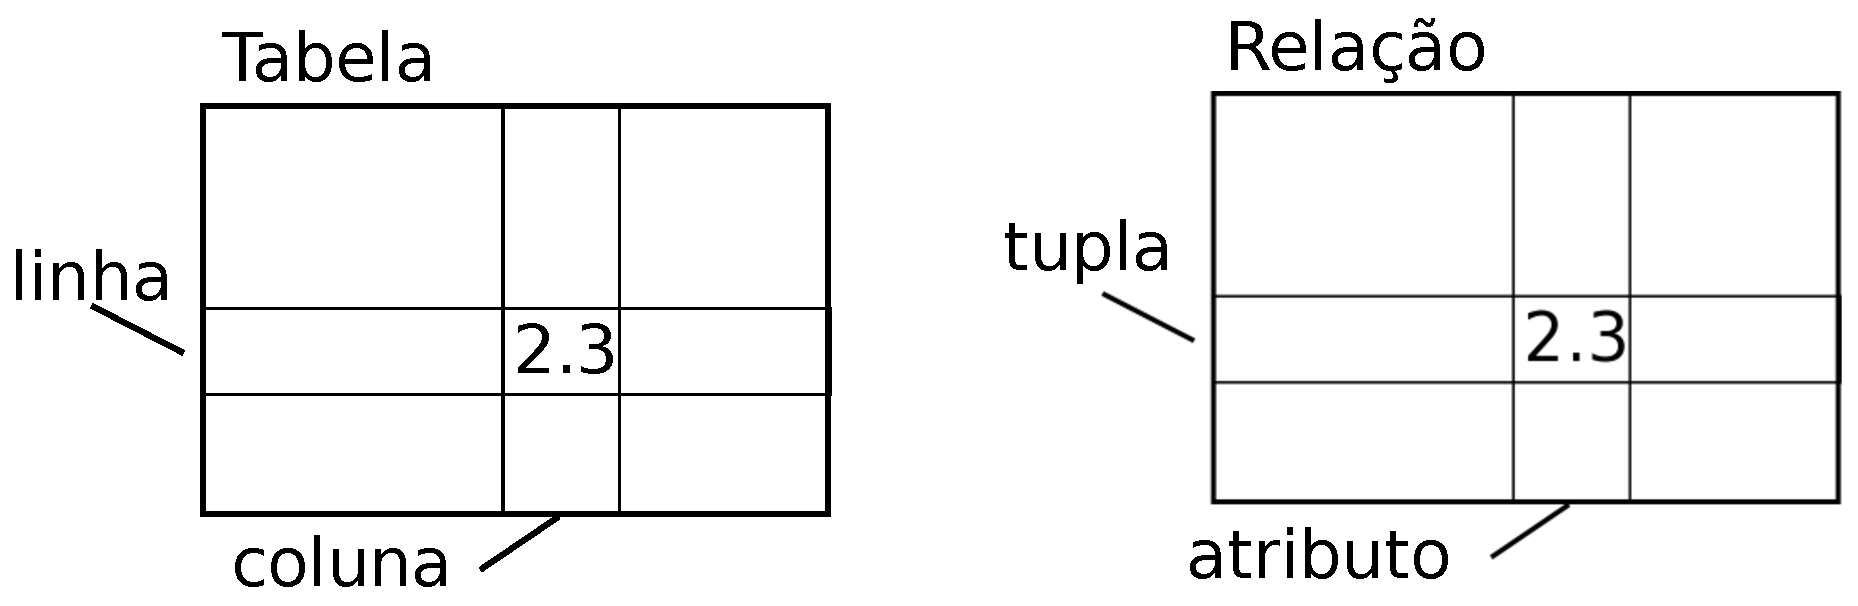
\includegraphics[height=1.50in]{figs2/relational.eps}}
\afterfig

%In technical descriptions of relational databases the concepts of 
%table, row, and column are more formally referred
%to as {\bf relation}, {\bf tuple}, and {\bf attribute}, respectively.
%We will use the less formal terms in this chapter.

Na descrição técnica de um banco de dados relacional o conceito de
tabela, linha e coluna são referências formais para {\bf relação},
{\bf tupla}, e {\bf atributo}, respectivamente.
Usaremos os termos menos formais neste capítulo.

%\section{SQLite manager Firefox add-on}
\section{Plugin do Firefox de Gerenciamento do SQLite}
%While this chapter will focus on using Python to work with data 
%in SQLite database files, many operations can be done more
%conveniently using a Firefox add-on called the {\bf SQLite
%  Database Manager} which is freely available from:

O foco deste capítulo é o uso do Python para trabalhar com dados
com o SQLite, muitas operações podem ser feitas de forma mais
conveniente utilizando um {\it plugin} do Firefox, o {\bf SQLite
  Database Manager} que está disponível gratuitamente através do {\it link}:

\url{https://addons.mozilla.org/en-us/firefox/addon/sqlite-manager/}

%Using the browser you can easily create tables, insert data, edit data, 
%or run simple SQL queries on the data in the database.

Utilizando o navegador você pode facilmente criar tabelas, inserir, editar ou
executar consultas SQL nos dados da base de dados.

%In a sense, the database manager is similar to a text editor
%when working with text files.   When you want to do one or
%very few operations on a text file, you can just open it
%in a text editor and make the changes you want.   When you have 
%many changes that you need to do to a text file, often you 
%will write a simple Python program.  You will find the same 
%pattern when working with databases.  You will do simple
%operations in the database manager and more complex operations
%will be most conveniently done in Python.

De certa forma, o gerenciador de banco de dados é similar a um editor de texto
quando trabalha com arquivos de texto. Quando você quer fazer uma ou mais
operações com um arquivo de texto, você pode simplesmente abrir o arquivo em
um editor de texto e fazer as alterações que desejar. Quando você tem
muitas alterações para fazer, normalmente você pode escrever um simples programa em 
Python para executar esta tarefa. Você encontrará os mesmos padrões
quando for trabalhar com banco de dados. Você fará operações em um gerenciador
de banco de dados e as operações mais complexas serão mais convenientes se
forem feitas com Python.

%\section{Creating a database table}
\section{Criando uma tabela em um banco de dados}

%Databases require more defined structure than Python lists 
%or dictionaries\footnote{SQLite actually does allow some 
%flexibility in the type of data stored in a column,
%but we will keep our data types strict in this chapter
%so the concepts apply equally to other database systems 
%such as MySQL.}.

Bancos de dados precisam de estruturas mais bem definidas do que listas ou
dicionários em Python\footnote{Atualmente o SQLite permite uma maior
  flexibilidade em relação aos tipos de dados que são armazenados em uma
  coluna, mas vamos manter os tipos de dados restritos neste capítulo, assim
  os mesmos conceitos aprendidos aqui podem ser aplicados a outros sistemas
  de banco de dados como MySQL.}.

%When we create a database {\bf table} we
%must tell the database in advance the names of each of the
%{\bf columns} in the table and the type of data which we are 
%planning to store in each {\bf column}.   When the database software
%knows the type of data in each column, it can choose the most 
%efficient way to store and look up the data based on the type of
%data.

Quando criamos uma {\bf tabela} em um banco de dados, precisamos informar ao
banco de dados previamente o nome de cada {\bf coluna} na tabela e o tipo de
dados que planejamos armazenar em cada {\bf coluna}. Quando o sistema de
banco de dados conhece o tipo de dado em cada coluna, ele pode definir a
forma mais eficiente de armazenar e consultar o dado baseado no tipo do dado.

%You can look at the various data types supported by SQLite
%at the following url:

Você pode visualizar os diversos tipos de dados que são suportados pelo SQLite
através do seguinte endereço:

\url{http://www.sqlite.org/datatypes.html}


%Defining structure for your data up front may seem inconvenient
%at the beginning, but the payoff is fast access to your data 
%even when the database contains a large amount of data.

Definir a estrutura dos seus tipos de dados pode parecer inconveniente no
começo, mas a recompensa é o acesso rápido aos dados mesmo quando o banco
de dados contém um grande número de informações.

%The code to create a database file and a table 
%named {\tt Tracks} with two columns in the 
%database is as follows:

O seguinte código cria um arquivo de banco de dados com uma tabela, chamada
{\tt Tracks}, contendo duas colunas:

\index{sqlite3 module}
\index{module!sqlite3}
\beforeverb
\begin{verbatim}
import sqlite3

conn = sqlite3.connect('music.sqlite3')
cur = conn.cursor()

cur.execute('DROP TABLE IF EXISTS Tracks ')
cur.execute('CREATE TABLE Tracks (title TEXT, plays INTEGER)')

conn.close()
\end{verbatim}
\afterverb
%
\index{connect function}
\index{function!connect}
\index{cursor function}
\index{function!cursor}
%The {\tt connect} operation makes a ``connection'' to the database 
%stored in the file {\tt music.sqlite3} in the current directory.   If
%the file does not exist, it will be created.  The reason this
%is called a ``connection'' is that sometimes the database is stored
%on a separate ``database server'' from the server on which we 
%are running our application.  In our simple examples 
%the database will just be a local file in the same directory
%as the Python code we are running.

A operação {\tt connect} cria uma ``conexão'' com o banco de dados armazenado
no arquivo {\tt music.sqlite3} no diretório corrente. Se o arquivo não
existir, este será criado. O motivo para isto ser chamado de ``conexão'' é
que algumas vezes o banco de dados está  em um ``servidor de banco de dados'' 
separado da aplicação propriamente dita. Em nossos exemplos o banco de dados
está armazenado localmente em um arquivo no mesmo diretório que o código
Python está sendo executado.


%A {\bf cursor} is like a file handle that we can use to perform
%operations on the data stored in the database.  Calling 
%{\tt cursor()} is very similar conceptually to calling
%{\tt open()} when dealing with text files.

Um {\bf cursor} é como um identificador de arquivo que podemos utilizar para
realizar operações sobre as informações armazenadas em um banco de dados. Ao
chamar a função {\tt cursor()}, conceitualmente, é similar ao chamar a função
{\tt open()} quando estamos trabalhando com arquivos de texto.

\beforefig
\centerline{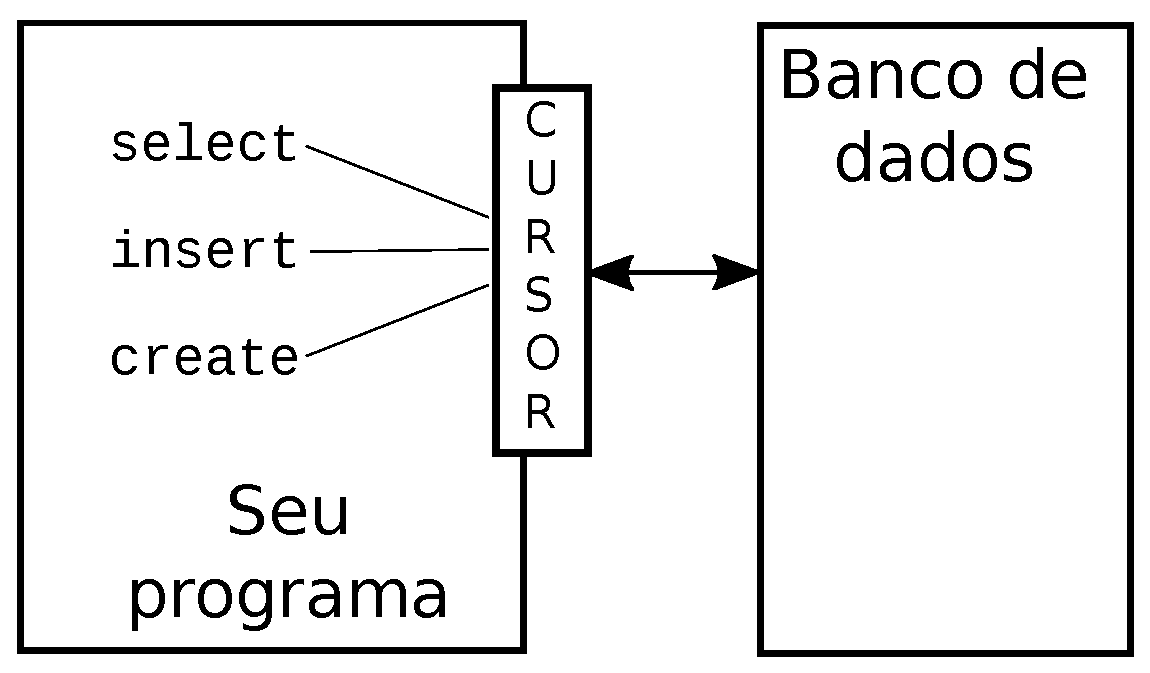
\includegraphics[height=1.50in]{figs2/cursor.eps}}
\afterfig

%Once we have the cursor, we can begin to execute 
%commands on the contents of the database using the {\tt execute()}
%method.

Uma vez que temos o cursor, podemos começar a executar comandos no conteúdo
armazenado no banco de dados utilizando o método {\tt execute()}.

%Database commands are expressed in a special language that has 
%been standardized across many different database vendors 
%to allow us to learn a single database language.   The database
%language is called {\bf Structured Query Language} or {\bf SQL}
%for short.

Os comandos de um banco de dados são expressos em uma linguagem especial que
foi padronizada por diferentes fornecedores de bancos de dados, que nos
permite aprender uma única linguagem. A linguagem dos bancos de dados é
chamada de {\bf Structured Query Language}\footnote{Em Português, pode ser
  chamada de Linguagem de Consulta Estruturada} ou referenciada pelo acrônimo
{\bf SQL}
\url{http://en.wikipedia.org/wiki/SQL}

%In our example, we are executing two SQL commands in our database.
%As a convention, we will show the SQL keywords in uppercase 
%and the parts of the command that we are adding (such as the
%table and column names) will be shown in lowercase.

Em nossos exemplos, estamos executando dois comandos SQL no banco de dados que
criamos. Convencionaremos que os comandos SQL serão mostrados em maiúsculas e
as partes que não são palavras reservadas do SQL (como os nomes das tabelas e
colunas) serão mostrados em minúsculas.

%The first SQL command removes the {\tt Tracks} table from the 
%database if it exists.  This pattern is simply to allow us to 
%run the same program to create the {\tt Tracks} table over 
%and over again without causing an error.  Note that the
%{\tt DROP TABLE} command deletes the table and all of its contents
%from the database (i.e., there is no ``undo'').

O primeiro comando SQL remove a tabela {\tt Tracks} do banco de dados se ela
existir. Este padrão nos permite executar o mesmo programa para criar a tabela
{\tt Tracks} repetidas vezes sem que cause erro. Perceba que o comando {\tt DROP
  TABLE} remove a tabela e todo o seu conteúdo do banco de dados (i.e., não é
possível desfazer esta operação)

\beforeverb
\begin{verbatim}
cur.execute('DROP TABLE IF EXISTS Tracks ')
\end{verbatim}
\afterverb
%
%The second command creates a table named
%{\tt Tracks} with a text column named {\tt title}
%and an integer column named {\tt plays}.
%
O segundo comando cria a tabela {\tt Tracks} com uma coluna chamada {\tt title}
com o tipo texto e uma coluna chamada {\tt plays} com o tipo inteiro.

\beforeverb
\begin{verbatim}
cur.execute('CREATE TABLE Tracks (title TEXT, plays INTEGER)')
\end{verbatim}
\afterverb
%
%Now that we have created a table named {\tt Tracks}, we can put some data
%into that table using the SQL {\tt INSERT} operation.   Again, we begin
%by making a connection to the database and obtaining the {\tt cursor}.
%We can then execute SQL commands using the cursor.
%
Agora que criamos a tabela {\tt Tracks}, podemos inserir algum dado dentro
dela utilizando a operação SQL {\tt INSERT}. Novamente, estamos
estabelecendo uma conexão com o banco de dados e obtendo o {\tt cursor}.
E então executamos o comando SQL utilizando o cursor.

%The SQL {\tt INSERT} command indicates which table we are using 
%and then defines a new row by listing the fields we want to 
%include {\tt (title, plays)} followed by the {\tt VALUES} we want
%placed in the new row.  We specify the values as question marks
%{\tt (?, ?)} to indicate that the actual values are passed in as a
%tuple {\tt ( 'My Way', 15 ) } as the second parameter to the
%{\tt execute()} call.

O comando SQL {\tt INSERT} indica qual tabela estamos utilizando, e em seguida, 
cria uma nova linha listando quais campos utilizaremos para incluir {\tt (title,
  plays)} seguido pelo comando {\tt VALUES} com os valores que desejamos
adicionar na nova linha. Especificamos os valores utilizando pontos de
interrogação {\tt (?, ?)} para indicar que os valores serão passados como
tuplas {\tt ( 'My Way', 15) } como um segundo parâmetro da chamada
{\tt execute()}.

\beforeverb
\begin{verbatim}
import sqlite3

conn = sqlite3.connect('music.sqlite3')
cur = conn.cursor()

cur.execute('INSERT INTO Tracks (title, plays) VALUES ( ?, ? )', 
    ( 'Thunderstruck', 20 ) )
cur.execute('INSERT INTO Tracks (title, plays) VALUES ( ?, ? )', 
    ( 'My Way', 15 ) )
conn.commit()

print 'Tracks:'
cur.execute('SELECT title, plays FROM Tracks')
for row in cur :
   print row

cur.execute('DELETE FROM Tracks WHERE plays < 100')
conn.commit()

cur.close()
\end{verbatim}
\afterverb
%
%First we {\tt INSERT} two rows into our table and use {\tt commit()} 
%to force the data to be written to the database file.

Primeiro nós adicionamos com {\tt INSERT} duas linhas na nossa tabela e
usaremos {\tt commit()} para forçar a escrita da informação no arquivo do banco
de dados.

\beforefig
\centerline{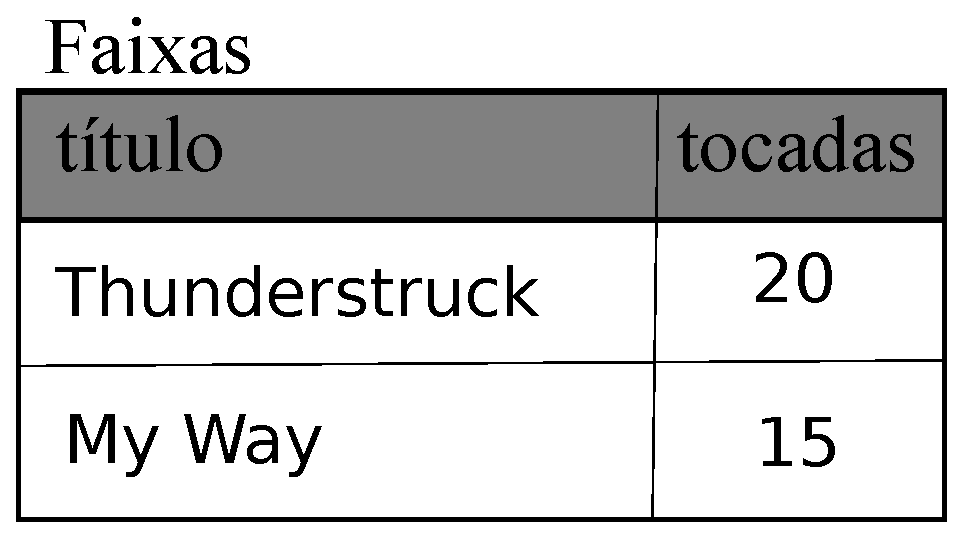
\includegraphics[height=1.00in]{figs2/tracks.eps}}
\afterfig

%Then we use the {\tt SELECT} command
%to retrieve the rows we just inserted from the table.  
%On the 
%{\tt SELECT} command, we indicate which columns we would like {\tt (title, plays)}
%and indicate which table we want to retrieve the data from.  After we 
%execute the {\tt SELECT} statement, the cursor is something we can loop through
%in a {\tt for} statement.   For efficiency,
%the cursor does not read all of the data from the
%database when we execute the {\tt SELECT} statement.  
%Instead, the data is read on demand
%as we loop through the rows in the {\tt for} statement.

Depois usamos o comando {\tt SELECT} para buscar a linha que acabamos de
inserir na tabela. Com o comando {\tt SELECT}, indicamos que coluna gostaríamos
{\tt (title, plays)} e de qual tabela queremos buscar a informação. Depois
de confirmar a execução do comando {\tt SELECT}, o cursor pode ser utilizado
como repetição através de um comando {\tt for}. Por questões de eficiência, o
cursor não lê toda a informação da base de dados quando executamos o comando
{\tt SELECT}. Ao invés disto, a informação é lida sob demanda enquanto
iteramos através da linha com o comando {\tt for}.

%The output of the program is as follows:

A saída do programa fica da seguinte forma:

\beforeverb
\begin{verbatim}
Tracks:
(u'Thunderstruck', 20)
(u'My Way', 15)
\end{verbatim}
\afterverb
%
\index{Unicode}
%Our {\tt for} loop finds two rows, and each row is a Python tuple with the
%first value as the {\tt title} and the second value as the number of {\tt plays}.
%Do not be concerned that the title strings are shown starting with 
%{\tt u'}.  This is an indication that the strings are {\bf Unicode} strings
%that are capable of storing non-Latin character sets.

A iteração do {\tt for} encontrou duas linhas, e cada linha é uma tupla em
Python com o primeiro valor como {\tt title} e o segundo como o número de
{\tt plays}. Não se preocupe com o fato de que {\it strings} são mostrados com
o caractere {\tt u'} no começo. Isto é uma indicação que a {\it string} estão
em {\bf Unicode}, o que indica que são capazes de armazenar um conjunto de
caractere não-Latin.

%At the very end of the program, we execute an SQL command to {\tt DELETE} 
%the rows we have just created so we can run the program over and over.
%The {\tt DELETE} command shows the use of a {\tt WHERE} clause that
%allows us to express a selection criterion so that we can ask the database
%to apply the command to only the rows that match the criterion.  In this example
%the criterion happens to apply to all the rows so we empty the table
%out so we can run the program repeatedly.  After the {\tt DELETE} is performed,
%we also call {\tt commit()} to force the data to be removed from the database.

No final do programa, executamos o comando SQL {\tt DELETE} para remover as
linhas que acabamos de criar, assim podemos executar o programa repetidas
vezes. O {\tt DELETE} pode ser utilizado com a condição {\tt WHERE} que permite
selecionar através de uma expressão o critério permitindo pesquisar no banco
de dados somente as linhas que correspondem com a expressão utilizada. Neste
exemplo a expressão construida se aplica em todas as linhas, para que possamos
executar o programa outras vezes. Depois de executar o {\tt DELETE} chamamos o
{\tt commit()} para forçar que o dado seja removido do banco de dados.

%\section{Structured Query Language summary}
\section{Resumo de Structured Query Language (SQL)}

%So far, we have been using the Structured Query Language in our Python
%examples and have covered many of the basics of the SQL commands.
%In this section, we look at the SQL language in particular
%and give an overview of SQL syntax.

Estamos utilizando SQL junto com os exemplos de Python e até agora cobrimos
muitos comandos SQL básicos. Nesta seção, vamos olhar a linguagem SQL com
mais atenção e apresentaremos uma visão geral da sintaxe do SQL.

%Since there are so many different database vendors, the Structured Query
%Language (SQL) was standardized so we could communicate in a portable
%manner to database systems from multiple vendors.

Existem diferentes fornecedores de bancos de dados, a linguagem SQL foi
padronizada, desta forma podemos nos comunicar de maneira portável entre os
diferentes sistemas de banco de dados dos diferentes fornecedores.

%A relational database is made up of tables, rows, and columns.  The columns
%generally have a type such as text, numeric, or date data.  When we create
%a table, we indicate the names and types of the columns:

Basicamente um banco de dados relacional é composto por tabelas, linhas e
colunas. As colunas geralmente possuem tipos, como textos, números ou
informação de data. Quando criamos uma tabela, indicamos os nomes e tipos das
colunas:

\beforeverb
\begin{verbatim}
CREATE TABLE Tracks (title TEXT, plays INTEGER)
\end{verbatim}
\afterverb
%
%To insert a row into a table, we use the SQL {\tt INSERT} command:
%
Para inserir uma linha em uma tabela, utilizamos o comando SQL {\tt INSERT}:

\beforeverb
\begin{verbatim}
INSERT INTO Tracks (title, plays) VALUES ('My Way', 15)
\end{verbatim}
\afterverb
%
%The {\tt INSERT} statement specifies the table name, then a list of
%the fields/columns that you would like to set in the new row, and then 
%the keyword {\tt VALUES} and a list of corresponding values 
%for each of the fields.
%
A declaração do {\tt INSERT} especifica o nome da tabela, e então, uma lista
dos campos/colunas que gostaríamos de definir na nova linha, e por fim,
através do campo {\tt VALUES} passamos uma lista de valores correspondentes a
cada campo.

%The SQL {\tt SELECT} command is used to retrieve rows and columns from a database.
%The {\tt SELECT} statement lets you specify which columns you would
%like to retrieve as well as a {\tt WHERE} clause to select which 
%rows you would like to see.  It also allows an optional 
%{\tt ORDER BY} clause to control the sorting of the returned rows.

O comando {\tt SELECT} é utilizado para buscar as linhas e colunas de um banco
de dados. A declaração do {\tt SELECT} permite que você especifique qual coluna
gostaria de buscar, bem como utilizando a condição do {\tt WHERE}, permite
selecionar qual linha gostaríamos de visualizar. Isto também possibilita o uso
de uma condição opcional, {\tt ORDER BY}, para ordenar as linhas retornadas.

\beforeverb
\begin{verbatim}
SELECT * FROM Tracks WHERE title = 'My Way'
\end{verbatim}
\afterverb
%
%Using \verb"*" indicates that you want the database to return all of 
%the columns for each row that matches the {\tt WHERE} clause.

O uso do \verb"*" indica que o banco de dados deve retornar todas as colunas
para cada linha que casa com a condição {\tt WHERE}.

%Note, unlike in Python, in a SQL {\tt WHERE} clause 
%we use a single equal sign 
%to indicate a test for equality rather than a double equal sign.
%Other logical operations allowed in a {\tt WHERE} clause include

Atenção, diferente de Python, a condição {\tt WHERE}, em SQL, utiliza o sinal
de igual simples (\verb"="), para indicar uma condição de igualdade, ao invés de
um sinal duplo (\verb"==")
\verb"<",
\verb">",
\verb"<=",
\verb">=",
\verb"!=",
%as well as {\tt AND} and {\tt OR} and parentheses
%to build your logical expressions.

assim como é possível utilizar as condições {\tt AND} e {\tt OR} e parênteses
para construir expressões lógicas.

%You can request that the returned rows be sorted by one of 
%the fields as follows:

Você pode pedir que as linhas retornadas sejam ordenadas por um dos campos
como apresentados no exemplo a seguir:
\beforeverb
\begin{verbatim}
SELECT title,plays FROM Tracks ORDER BY title
\end{verbatim}
\afterverb
%
%To remove a row, you need a {\tt WHERE} clause on an SQL {\tt DELETE}
%statement.  The {\tt WHERE} clause determines which rows are to be deleted:
%
Para remover uma linha, é preciso combinar a condição {\tt WHERE} com a
condição {\tt DELETE}. O {\tt WHERE} irá determinar quais linhas serão
removidas:

\beforeverb
\begin{verbatim}
DELETE FROM Tracks WHERE title = 'My Way'
\end{verbatim}
\afterverb
%
%It is possible to {\tt UPDATE} a column or columns within one or more rows
%in a table using the SQL {\tt UPDATE} statement as follows:
%
É possível alterar/atualizar uma ou mais colunas e suas linhas de uma tabela
utilizando a condição SQL {\tt UPDATE}, da seguinte forma:

\beforeverb
\begin{verbatim}
UPDATE Tracks SET plays = 16 WHERE title = 'My Way'
\end{verbatim}
\afterverb
%
%The {\tt UPDATE} statement specifies a table and 
%then a list of fields and values to change after the {\tt SET} 
%keyword and then an optional {\tt WHERE} clause to select
%the rows that are to be updated.  A single {\tt UPDATE} statement
%will change all of the rows that match the {\tt WHERE} clause.  If 
%a {\tt WHERE} clause is not specified, it performs the {\tt UPDATE}
%on all of the rows in the table.
%
A condição {\tt UPDATE} especifica uma tabela e depois uma lista de campos e
valores que serão alterados após o comando {\tt SET}, e utilizando uma condição
{\tt WHERE}, opcional, é possível selecionar as linhas que serão atualizadas.
Uma condição {\tt UPDATE} irá mudar todas as linhas que casam com a condição
{\tt WHERE}. Se a condição {\tt WHERE} não for especificada, o {\tt UPDATE}
será aplicado em todas as linhas da tabela.

%These four basic SQL commands (INSERT, SELECT, UPDATE, and DELETE) allow 
%the four basic operations needed to create and maintain data.

Os quatro comandos básicos de SQL (INSERT, SELECT, UPDTE e DELETE) permitem
as quatro operações básicas necessárias para criação e manutenção das
informações em um banco de dados.

%\section{Spidering Twitter using a database}
\section{Rastreando o Twitter utilizando um banco de dados}

%In this section, we will create a simple spidering program that will 
%go through Twitter accounts and build a database of them.
%\emph{Note: Be very careful when running this program.  You do not
%want to pull too much data or run the program for too long and
%end up having your Twitter access shut off.}

Nesta seção, criaremos um programa simples para rastreamento que navegará
através de contas de usuários do Twitter e construirá um banco de dados
referentes a estes usuários.
\emph{Nota: Tenha muito cuidado ao executar este programa. Você não irá querer
  extrair muitas informações ou executar o programa por muito tempo e acabar
  tendo sua conta do Twitter bloqueada.}

%One of the problems of any kind of spidering program is that it 
%needs to be able to be stopped and restarted many times and 
%you do not want to lose the data that you have retrieved so far.
%You don't want to always restart your data retrieval at the
%very beginning so we want to store data as we retrieve it so our
%program can start back up and pick up where it left off.

Um dos problemas, em qualquer tipo de programas de rastreamento, é que precisa
ser capaz de ser interrompido e reiniciado muitas vezes e você não quer perder
informações que você já tenha recuperado até agora. Não quer sempre reiniciar
a recuperação dos dados desde o começo, então armazenamos as informações tão
logo seja recuperada, assim o programa poderá reiniciar a busca do ponto onde
parou.

%We will start by retrieving one person's Twitter friends and their
%statuses, looping through the list of friends, and adding each 
%of the friends to a database to be retrieved in the future.  After
%we process one person's Twitter friends, we check in our database
%and retrieve one of the friends of the friend.  We do this over and
%over, picking an ``unvisited'' person, retrieving their friend list,
%and adding friends we have not seen to our list for a future visit.

Vamos começar recuperando os amigos de uma pessoa no Twitter e seus status,
iterando na lista de amigos, e adicionando cada um ao banco de dados para
que possa ser recuperado no futuro. Depois de listar os amigos de uma pessoa,
verificamos na nossa base de dados e coletamos os amigos de um dos amigos da
primeira pessoa. Vamos fazendo isto repetidas vezes, escolhendo umas das
pessoas ``não visitadas'', recuperando sua lista de amigos, e
adicionando amigos que não tenhamos visto anteriormente a nossa lista, para
visitar futuramente.

%We also track how many times we have seen a particular friend in the
%database to get some sense of their ``popularity''.

Também rastrearemos quantas vezes vimos um amigo em particular na nossa base
para ter uma ideia da sua ``popularidade''.

%By storing our list of known accounts and whether 
%we have retrieved the account or not, 
%and how popular the account is in a database on the disk
%of the computer, we can stop and
%restart our program as many times as we like.

Armazenando nossa lista de contas conhecidas, no banco de dados no disco do
nosso computador, e se já recuperamos a conta ou não, e quanto esta conta é
popular, podemos parar e recomeçar nosso programa quantas vezes quisermos.

% TODO: Add a reference to the right spot
%This program is a bit complex. It is based on the code 
%from the exercise earlier in the book that uses
%the Twitter API.

% TODO: Adicionar a referência do código para o lugar certo.
Este programa é um pouco complexo. É baseado em um exercício apresentado
anteriormente neste livro, que utiliza a API do Twitter.

%Here is the source code for our Twitter spidering application:

O seguinte código apresenta o programa que realiza o rastreamento no Twitter:

\beforeverb
\begin{verbatim}
import urllib
import twurl
import json
import sqlite3

TWITTER_URL = 'https://api.twitter.com/1.1/friends/list.json'

conn = sqlite3.connect('spider.sqlite3')
cur = conn.cursor()

cur.execute('''
CREATE TABLE IF NOT EXISTS Twitter 
(name TEXT, retrieved INTEGER, friends INTEGER)''')

while True:
    acct = raw_input('Enter a Twitter account, or quit: ')
    if ( acct == 'quit' ) : break
    if ( len(acct) < 1 ) :
        cur.execute('SELECT name FROM Twitter WHERE retrieved = 0 LIMIT 1')
        try:
            acct = cur.fetchone()[0]
        except:
            print 'No unretrieved Twitter accounts found'
            continue

    url = twurl.augment(TWITTER_URL, 
               {'screen_name': acct, 'count': '20'} )
    print 'Retrieving', url
    connection = urllib.urlopen(url)
    data = connection.read()
    headers = connection.info().dict
    # print 'Remaining', headers['x-rate-limit-remaining']
    js = json.loads(data)
    # print json.dumps(js, indent=4)

    cur.execute('UPDATE Twitter SET retrieved=1 WHERE name = ?', (acct, ) )

    countnew = 0
    countold = 0
    for u in js['users'] :
        friend = u['screen_name']
        print friend
        cur.execute('SELECT friends FROM Twitter WHERE name = ? LIMIT 1', 
            (friend, ) )
        try:
            count = cur.fetchone()[0]
            cur.execute('UPDATE Twitter SET friends = ? WHERE name = ?', 
                (count+1, friend) )
            countold = countold + 1
        except:
            cur.execute('''INSERT INTO Twitter (name, retrieved, friends) 
                VALUES ( ?, 0, 1 )''', ( friend, ) )
            countnew = countnew + 1
    print 'New accounts=',countnew,' revisited=',countold
    conn.commit()

cur.close()
\end{verbatim}
\afterverb
%
%Our database is stored in the file {\tt spider.sqlite3} and it has one 
%table named {\tt Twitter}.  Each row in the {\tt Twitter} table
%has a column for the account name, whether we have retrieved the friends
%of this account, and how many times this account has been ``friended''.

%
Nossa base de dados está armazenada no arquivo {\tt spider.sqlite3} e possui
uma tabela chamada {\tt Twitter}. Cada linha na tabela {\tt Twitter} tem uma
coluna para o nome da conta, se já recuperamos os amigos desta conta, e quantas
vezes esta conta foi ``seguida''.

%In the main loop of the program, we prompt the user for a Twitter
%account name or ``quit'' to exit the program.  
%If the user enters a Twitter account, we retrieve the 
%list of friends and statuses
%for that user and add each friend to the database if 
%not already in the database.  If the friend is already in the list, 
%we add 1 to the {\tt friends} field in the row in the database.

Na repetição principal do programa, pedimos ao usuário uma conta de Twitter
ou ``quit'' para sair do programa. Se o usuário informar um usuário do Twitter,
o programa começa a recuperar a lista de amigos e os status para aquele
usuário e adiciona cada amigo na base de dados, se ainda não existir. Se o amigo já
está na lista, nós adicionamos ``1'' no campo {\tt friends} da base de dados.


%If the user presses enter, we look in the database for the next 
%Twitter account that we have not yet retrieved, retrieve the
%friends and statuses for that account, add them to the database 
%or update them, and increase their {\tt friends} count.

Se o usuário pressionar {\tt enter}, pesquisamos na base a próxima conta que
não rastreamos ainda, e então rastreamos os amigos e status com aquela conta
e adicionamos na base de dados ou atualizamos, incrementando seu contador de
{\tt friends}.

%Once we retrieve the list of friends and statuses, we loop 
%through all of the {\tt user} items in the returned JSON
%and retrieve the \verb"screen_name" for each user.  Then we use
%the {\tt SELECT} statement to see if we already have stored this
%particular \verb"screen_name" in the database and retrieve the
%friend count ({\tt friends}) if the record exists.

Uma vez que rastreamos a lista de amigos e status, iteramos entre todas os
ítens {\tt user} retornados no JSON e rastreamos o  \verb"screen_name" para
cada usuário. Então utilizamos a declaração {\tt SELECT} para ver se já
armazenamos este \verb"screen_name" em particular na base e recuperamos o
contador de amigos ({\tt friends}), se este registro existir.

\beforeverb
\begin{verbatim}
    countnew = 0
    countold = 0
    for u in js['users'] :
        friend = u['screen_name']
        print friend
        cur.execute('SELECT friends FROM Twitter WHERE name = ? LIMIT 1', 
            (friend, ) )
        try:
            count = cur.fetchone()[0]
            cur.execute('UPDATE Twitter SET friends = ? WHERE name = ?', 
                (count+1, friend) )
            countold = countold + 1
        except:
            cur.execute('''INSERT INTO Twitter (name, retrieved, friends) 
                VALUES ( ?, 0, 1 )''', ( friend, ) )
            countnew = countnew + 1
    print 'New accounts=',countnew,' revisited=',countold
    conn.commit()
\end{verbatim}
\afterverb
%
%Once the cursor executes the {\tt SELECT} statement, 
%we must retrieve the rows.  We could do this with a {\tt for} 
%statement, but since we are only retrieving
%one row ({\tt LIMIT 1}), we can use the {\tt fetchone()} method to fetch the
%first (and only) row that is the result of the {\tt SELECT} operation.  
%Since {\tt fetchone()} returns the row as a {\bf tuple} (even though there is only
%one field), we take the first value from the tuple using {\tt [0]} to get the 
%current friend count into the variable {\tt count}.  

%
Uma vez que o cursor tenha executado o {\tt SELECT}, nós devemos recuperar as
linhas. Podemos fazer isto com uma declaração de {\tt for}, mas uma vez que
estamos recuperando uma linha ({\tt LIMIT 1}), podemos utilizar o método
{\tt fetchone()} para buscar a primeira (e única) linha que é o resultado da
operação {\tt SELECT}. Sendo o retorno {\tt fetchone()} uma linha como uma
{\bf tupla} (ainda que haja somente um campo), pegamos o primeiro valor da
tupla utilizando índice {\tt [0]} para pegar o contador de amigos atual dentro
da variável {\tt count}.

%If this retrieval is successful, we use the SQL {\tt UPDATE} statement with a 
%{\tt WHERE} clause to add 1 to the {\tt friends} column for the row that 
%matches the friend's account.  Notice that there are two placeholders (i.e.,
%question marks) in the SQL, and the second parameter to the {\tt execute()} is
%a two-element tuple that holds the values to be substituted into the SQL
%in place of the question marks.

Se a busca for bem sucedida, utilizamos a declação {\tt UPDATE} com a cláusula 
{\tt WHERE} para adicionar 1 na coluna {\tt friends} para a linha que
corresponde com a conta do amigo. Note que existem dois espaços reservados
(i.e., pontos de interrogações) no SQL, e o segundo parâmetro para o
{\tt execute()} é uma tupla que armazena o valor para substituir no SQL no
lugar dos pontos de interrogações.

%If the code in the {\tt try} block fails, it is probably because no record
%matched the {\tt WHERE name = ?} clause on the SELECT statement.  So in the
%{\tt except} block, we use the SQL {\tt INSERT} statement to add the friend's
%\verb"screen_name" to the table with an indication that we have not yet 
%retrieved the \verb"screen_name" and set the friend count to zero.

Se o bloco {\tt try} falhar, é provavelmente por que nenhum resultado
corresponde a cláusula em {\tt WHERE name = ?} do SELECT. Então no block
{\tt except}, utilizamos a declaração {\tt INSERT} para adicionar o
\verb"screen_name" do amigo a tabela com a indicação que ainda não rastreamos
o \verb"screen_name" e setamos o contador de amigos com 0 (zero).

%So the first time the program runs and we enter a Twitter account, the program
%runs as follows:

Assim, a primeira vez que o programa é executado e informamos uma conta do
Twitter, a saída do programa é a seguinte:

\beforeverb
\begin{verbatim}
Enter a Twitter account, or quit: drchuck
Retrieving http://api.twitter.com/1.1/friends ...
New accounts= 20  revisited= 0
Enter a Twitter account, or quit: quit
\end{verbatim}
\afterverb
%
%Since this is the first time we have run the program, the database
%is empty and we create the database in the file {\tt spider.sqlite3} and
%add a table named {\tt Twitter} to the database.  Then we retrieve
%some friends and add them all to the database since the database is
%empty.

Como esta é a primeira vez que executamos o programa, o banco de dados está
vazio e criamos o banco no arquivo {\tt spider.sqlite3}, adicionamos a tabela
chamada {\tt Twitter} na base de dados. Então nós rastreamos alguns amigos e
os adicionamos a base, uma vez que ela está vazia.

%At this point, we might want to write a simple database dumper
%to take a look at what is in our {\tt spider.sqlite3} file:

Neste ponto podemos escrever um {\it dumper} simples para olhar o que está no
nosso arquivo {\tt spider.sqlite3}:

\beforeverb
\begin{verbatim}
import sqlite3

conn = sqlite3.connect('spider.sqlite3')
cur = conn.cursor()
cur.execute('SELECT * FROM Twitter')
count = 0
for row in cur :
   print row
   count = count + 1
print count, 'rows.'
cur.close()
\end{verbatim}
\afterverb
%
%This program simply opens the database and selects all of the 
%columns of all of the rows in the table {\tt Twitter}, then 
%loops through the rows and prints out each row.

Este programa abre o banco de dados e seleciona todas as colunas de todas as
linhas na tabela {\tt Twitter}, depois itera em cada linha e imprime o valor
dentro de cada uma.

%If we run this program after the first execution of our Twitter
%spider above, its output will be as follows:

Se executarmos este programa depois da primeira execução do nosso rastreador
{\it spider} do Twitter, sua saída será como a seguinte:

\beforeverb
\begin{verbatim}
(u'opencontent', 0, 1)
(u'lhawthorn', 0, 1)
(u'steve_coppin', 0, 1)
(u'davidkocher', 0, 1)
(u'hrheingold', 0, 1)
...
20 rows.
\end{verbatim}
\afterverb
%
%We see one row for each \verb"screen_name", that we 
%have not retrieved the data for that \verb"screen_name", and 
%everyone in the database has one friend.

Veremos uma linha para cada \verb"screen_name", que não tenhamos recuperado
o dado daquele \verb"screen_name", e todos tem um amigo.

%Now our database reflects the retrieval of the friends of 
%our first Twitter account ({\bf drchuck}).  We can run the program
%again and tell it to retrieve the friends of the next 
%``unprocessed'' account by simply pressing enter instead of
%a Twitter account as follows:

Agora nosso banco de dados reflete quais amigos estão relacionados com a nossa
primeira conta do Twitter ({\bf drchuck}) utilizada para rastreamento. Podemos
executar o programa novamente e mandar rastrear a próxima conta
``não processada'' e recuperar os amigos, simplesmente pressionando {\tt enter}
ao invés de informar uma conta do Twitter, conforme o exemplo a seguir:

\beforeverb
\begin{verbatim}
Enter a Twitter account, or quit: 
Retrieving http://api.twitter.com/1.1/friends ...
New accounts= 18  revisited= 2
Enter a Twitter account, or quit: 
Retrieving http://api.twitter.com/1.1/friends ...
New accounts= 17  revisited= 3
Enter a Twitter account, or quit: quit
\end{verbatim}
\afterverb
%
%Since we pressed enter (i.e., we did not specify a Twitter account),
%the following code is executed:

%
Uma vez que pressionamos {\tt enter} (i.e., não especificamos uma conta do
Twitter), o seguinte código é executado:

\beforeverb
\begin{verbatim}
    if ( len(acct) < 1 ) :
        cur.execute('SELECT name FROM Twitter WHERE retrieved = 0 LIMIT 1')
        try:
            acct = cur.fetchone()[0]
        except:
            print 'No unretrieved twitter accounts found'
            continue
\end{verbatim}
\afterverb
%
%We use the SQL {\tt SELECT} statement to retrieve the name of the first 
%({\tt LIMIT 1}) user who still has their ``have we retrieved this user''
%value set to zero.  We also use the {\tt fetchone()[0]} pattern within 
%a try/except block to either extract a \verb"screen_name" from the retrieved
%data or put out an error message and loop back up.

Utilizamos a declaração SQL {\tt SELECT} para recuperar o nome do primeiro
({\tt LIMIT 1}) usuário que ainda tem seu ``recuperamos este usuário'' com o
valor setado em zero. Também utilizamos o padrão {\tt fetchone()[0]} dentro de
um bloco try/except para extrair também um \verb"screen_name" do dado
recuperado ou apresentamos uma mensagem de erro e iteramos novamente.

%If we successfully retrieved an unprocessed \verb"screen_name", we retrieve
%their data as follows:

Se tivermos sucesso ao recuperar um \verb"screen_name" não processado, vamos
extrair seus dados da seguinte maneira:

\beforeverb
\begin{verbatim}
    url = twurl.augment(TWITTER_URL, {'screen_name': acct, 'count': '20'} )
    print 'Retrieving', url
    connection = urllib.urlopen(url)
    data = connection.read()
    js = json.loads(data)

    cur.execute('UPDATE Twitter SET retrieved=1 WHERE name = ?', (acct, ) )
\end{verbatim}
\afterverb
%
%Once we retrieve the data successfully, we use the {\tt UPDATE} statement 
%to set the {\tt retrieved} column to 1 to indicate that we have completed 
%the retrieval of the friends of this account.  This keeps us from retrieving
%the same data over and over and keeps us progressing forward through the network
%of Twitter friends.
%
Ao recuperar os dados com sucesso, utilizaremos a declaração {\tt UPDATE} para
setar a coluna {\tt retrieved} para 1 para indicar que completamos a extração
dos amigos relacionados com esta conta. Isto no permite recuperar o mesmo dado
diversas vezes e nos permite prosseguir através da lista de amigos no Twitter. 

%If we run the friend program and press enter twice to retrieve the next 
%unvisited friend's friends,
%then run the dumping program, it will give us the following output:

Se executarmos o programa novamente, e pressionarmos {\tt enter} duas vezes
seguidas para recuperar os próximos amigos do amigo e depois executarmos o
programa de {\it dumping}, ele nos mostrará a seguinte saída:

\beforeverb
\begin{verbatim}
(u'opencontent', 1, 1)
(u'lhawthorn', 1, 1)
(u'steve_coppin', 0, 1)
(u'davidkocher', 0, 1)
(u'hrheingold', 0, 1)
...
(u'cnxorg', 0, 2)
(u'knoop', 0, 1)
(u'kthanos', 0, 2)
(u'LectureTools', 0, 1)
...
55 rows.
\end{verbatim}
\afterverb
%
%We can see that we have properly recorded that we have visited 
%{\tt lhawthorn} and {\tt opencontent}.  Also the accounts 
%{\tt cnxorg} and {\tt kthanos} already have two followers.
%Since we now have retrieved the friends of three people
%({\tt drchuck}, {\tt opencontent}, and {\tt lhawthorn}) our table has 55 rows 
%of friends to retrieve.

KKKKKKKKKKKKKKKKKKKKKKKKKKKKKKKKKKKKKKKKKKKKKKKKKKKKKKKKKKKKKKKKKKKKKKKKKKKKKKKKKKKKKKKKKKKKKKKKKKK

Podemos ver que gravamos de forma apropriada que visitamos os usuários
{\tt lhawthorn} e {\tt opencontent}. E que as contas {\tt cnxorg} e
{\tt kthanos} já tem dois seguidores. Desde que tenhamos recuperado os amigos
de três pessoas ({\tt drchuck}, {\tt opencontent}, e {\tt lhawthorn}) nossa
tabela tem agora 55 linhas de amigos recuperados.

%Each time we run the program and press enter it will pick the next 
%unvisited account (e.g., the next account will be \verb"steve_coppin"),
%retrieve their friends, mark them as retrieved, and for each of the 
%friends of \verb"steve_coppin" either add them to the end of the 
%database or update their friend count if they are already in the
%database.

Cada vez que executamos o programa e pressionamos {\tt enter} ele pegará a
próxima conta não visitada (e.g., a próxima conta será \verb"steve_coppin"),
recuperar seus amigos, marcá-los como recuperados, e para cada um dos amigos
de \verb"steve_coppin" também adicionaremos eles para no fim da base de dados 
e atualizaremos seus amigos que já estiverem na base de dados.

%Since the program's data is all stored on disk in a database, 
%the spidering activity can be suspended and resumed as many times as you 
%like with no loss of data.

Assim que os dados do programa estejam armazenados no disco em um banco de
dados o rastreamento pode ser suspenso e reiniciado tantas vezes quando
quiser sem a perda de informações.

%\section{Basic data modeling}
\section{Modelagem de dados básica}

%The real power of a relational database is when we create multiple tables
%and make links between those tables.   The act of deciding how to break
%up your application data into multiple tables and establishing the
%relationships between the tables is called {\bf data modeling}.  The
%design document that shows the tables and their relationships 
%is called a {\bf data model}.

O verdadeiro poder de um banco de dados relacional é quando criamos múltiplas
tabelas e criamos ligações entre elas. Decidir como dividir os dados da sua
aplicação em diferentes tabelas e estabelecer a relação entre estas tabelas é
o que chamamos de {\bf modelagem de dados}. O documento que mostra a estrutura 
das tabelas e suas relações é chamado de {\bf modelo de dados}.

%Data modeling is a relatively sophisticated skill and we will only introduce
%the most basic concepts of relational data modeling in this section.  For more
%detail on data modeling you can start with:

Modelagem de dados é uma habilidade relativamente sofisticada e nesta seção
nós iremos somente introduzir os conceitos mais básicos da modelagem de dados
relacionais. Para maiores detalhes sobre modelagem de dados você pode começar
com:

\url{http://en.wikipedia.org/wiki/Relational_model}

%Let's say for our Twitter spider application, instead of just
%counting a person's friends, we wanted to keep a list of 
%all of the incoming relationships so we could find a list of 
%everyone who is following a particular account.

Digamos que para a nossa aplicação de rastreamento do Twitter, ao invés de
só contar os amigos das pessoas, nós queiramos manter uma lista de todas as
relações de entrada, então poderemos encontrar uma lista de todos que seguem
uma pessoa em particular.

%Since everyone will potentially have many accounts that follow
%them, we cannot simply add a single column to our {\tt Twitter} table. 
%So we create a new table that keeps track of pairs of friends.
%The following is a simple way of making such a table:

Já que todos, potencialmente, terão tantas contas que o sigam, nós não podemos
simplesmente adicionar uma coluna para nossa tabela {\tt Twitter}. Então
criamos uma nova tabela que mantém o controle dos pares de amigos. A seguir
temos uma forma simples de criar tal tabela:

\beforeverb
\begin{verbatim}
CREATE TABLE Pals (from_friend TEXT, to_friend TEXT)
\end{verbatim}
\afterverb
%
%Each time we encounter a person who {\tt drchuck} is following, we
%would insert a row of the form:
%
Toda vez que encontrarmos uma pessoa que {\tt drchuck} está seguindo, nós
iremos inserir uma linha da seguinte forma:

\beforeverb
\begin{verbatim}
INSERT INTO Pals (from_friend,to_friend) VALUES ('drchuck', 'lhawthorn')
\end{verbatim}
\afterverb
%
%As we are processing the 20 friends from the {\tt drchuck}
%Twitter feed, we will insert 20 records with ``drchuck''
%as the first parameter so we will end up duplicating the 
%string many times in the database.
%
Como estamos processando 20 amigos da conta do {\it Twitter} do {\tt drchuck},
inserimor 20 registros com ``drchuck'' como primeiro parâmetro e assim
acaberemos duplicando a {\it string} muitas vezes no banco de dados.

%This duplication of string data violates one of the best practices 
%for {\bf database normalization} which basically states that
%we should never put the same string data in the database more than once.  
%If we need the data more than once, we create a 
%numeric {\bf key} for the data and reference the actual data 
%using this key.

Esta duplicação de dados viola uma das melhores práticas da {\bf normatização
  de banco de dados} que basicamente afirma que nunca devemos colocar o mesmo
dado mais de uma vez em um banco de dados. Se precisarmos inserir um dado mais
de uma vez, criamos uma referência numérica {\bf key} (chave) para o dado, e
utilizamos a chave para referenciar o dado.

%In practical terms, a string takes up a lot more 
%space than an integer on the disk
%and in the memory of our computer, and takes more processor time
%to compare and sort.  If we only have a few hundred entries, 
%the storage and processor time hardly matters.  But if we have 
%a million people in our database and a possibility of 100 million
%friend links, it is important to be able to scan data as quickly
%as possible.

Na prática, uma {\it string} ocupa muito mais espaço do que um inteiro, no
disco e na memória do nosso computador, e leva mais tempo do processor para
comparar e ordenar. Se tivermos somente algumas centenas de entradas, a base
de dados e o tempo de processamento dificilmente importarão. Mas se tivermos
um milhão de pessoas na nossa base de dados e uma possibilidade de 100 milhões
de conexões de amigos, é importante permitir examinar os dados o mais rápido
possível.

%We will store our Twitter accounts in a table named {\tt People}
%instead of the {\tt Twitter} table used in the previous example.
%The {\tt People} table has an additional column 
%to store the numeric key associated with the 
%row for this Twitter user.   
%SQLite has a feature that automatically adds the key value
%for any row we insert into a table using a special type of 
%data column ({\tt INTEGER PRIMARY KEY}).

Nós armazenaremos nossas contas do Twitter em uma tabela chamada {\tt People}
ao invés de utilizar a tabela {\tt Twitter} utilizada no exemplo anterior. A
tabela {\tt People} tem uma coluna adicional para armazenar uma chave associada
a linha para este usuário.

%We can create the {\tt People} table with this additional 
%{\tt id} column as follows:

Podemos criar a tabela {\tt People} com esta coluna {\tt id} adicional com o
seguinte comando:

\beforeverb
\begin{verbatim}
CREATE TABLE People 
    (id INTEGER PRIMARY KEY, name TEXT UNIQUE, retrieved INTEGER)
\end{verbatim}
\afterverb
%
%Notice that we are no longer maintaining a friend count in each row
%of the {\tt People} table.
%When we select {\tt INTEGER PRIMARY KEY} as the type of our {\tt id} column,
%we are indicating that we would like SQLite to manage this column and 
%assign a unique numeric key to each row we insert automatically.
%We also add the keyword {\tt UNIQUE} to indicate that we will not 
%allow SQLite to insert two rows with the same value for {\tt name}.
%
Perceba que nós não estamos mais mantendo uma conta de amigo em cada linha da
tabela {\tt People}. Quando selecionamos {\tt INTEGER PRIMARY KEY} como o tipo
da nossa coluna {\tt id}, estamos indicando que gostaríamos que o SQLite
gerencie esta coluna e defina uma chave numérica única automagicamente para
cada linha que inserirmos. Também adicionamos uma palavra-chave {\tt UNIQUE}
para indicar que não permitiremos ao SQLite inserir duas linhas com o mesmo
valor para {\tt name}.

%Now instead of creating the table {\tt Pals} above, we create
%a table called {\tt Follows} with two integer columns
%\verb"from_id" and \verb"to_id" and a constraint on the table that
%the \emph{combination} of \verb"from_id" and \verb"to_id" must be unique 
%in this table (i.e., we cannot insert duplicate rows) in our database.

Agora, ao invés de criar a tabela {\tt Pals} acima, criaremos uma tabela
chamada {\tt Follows} com duas colunas com o tipo inteiro \verb"from_id" e
\verb"to_id" e associaremos na tabela onde a \emph{combinação} de
\verb"from_id" e \verb"to_id" devem ser únicos nesta tabela (i.e., não podemos
inserir linhas duplicadas) na nossa base de dados.

\beforeverb
\begin{verbatim}
CREATE TABLE Follows 
    (from_id INTEGER, to_id INTEGER, UNIQUE(from_id, to_id) )
\end{verbatim}
\afterverb
%
%When we add {\tt UNIQUE} clauses to our tables, we are communicating a set
%of rules that we are asking the database to enforce when we attempt to insert
%records.   We are creating these rules as a convenience in our programs, as we
%will see in a moment.  The rules both keep us from making mistakes and make
%it simpler to write some of our code.

Quando adicionamos a condição {\tt UNIQUE} a nossa tabela, estamos definindo
um conjunto de regras e pedindo a base de dados para cumprir estas regras
quando tentarmos inserir algum registro. Estamos criando estas regras como uma
conveniencia no nosso programa, como veremos a seguir. As regras nos impede de
cometer enganos e facilita na escrita dos nossos códigos.

%In essence, in creating this {\tt Follows} table, we are modelling a 
%``relationship'' where one person ``follows'' someone else
%and representing it with a pair of numbers indicating that (a) the people are
%connected and (b) the direction of the relationship.

Em essencia, criando a tabela {\tt Follows}, estamos modelando uma ``relação''
onde uma pessoa ``segue'' outro alguém e representamos isto com um par de
números indicando que (a) as pessoas estão conectadas e (b) a direção do
relacionamento.

\beforefig
\centerline{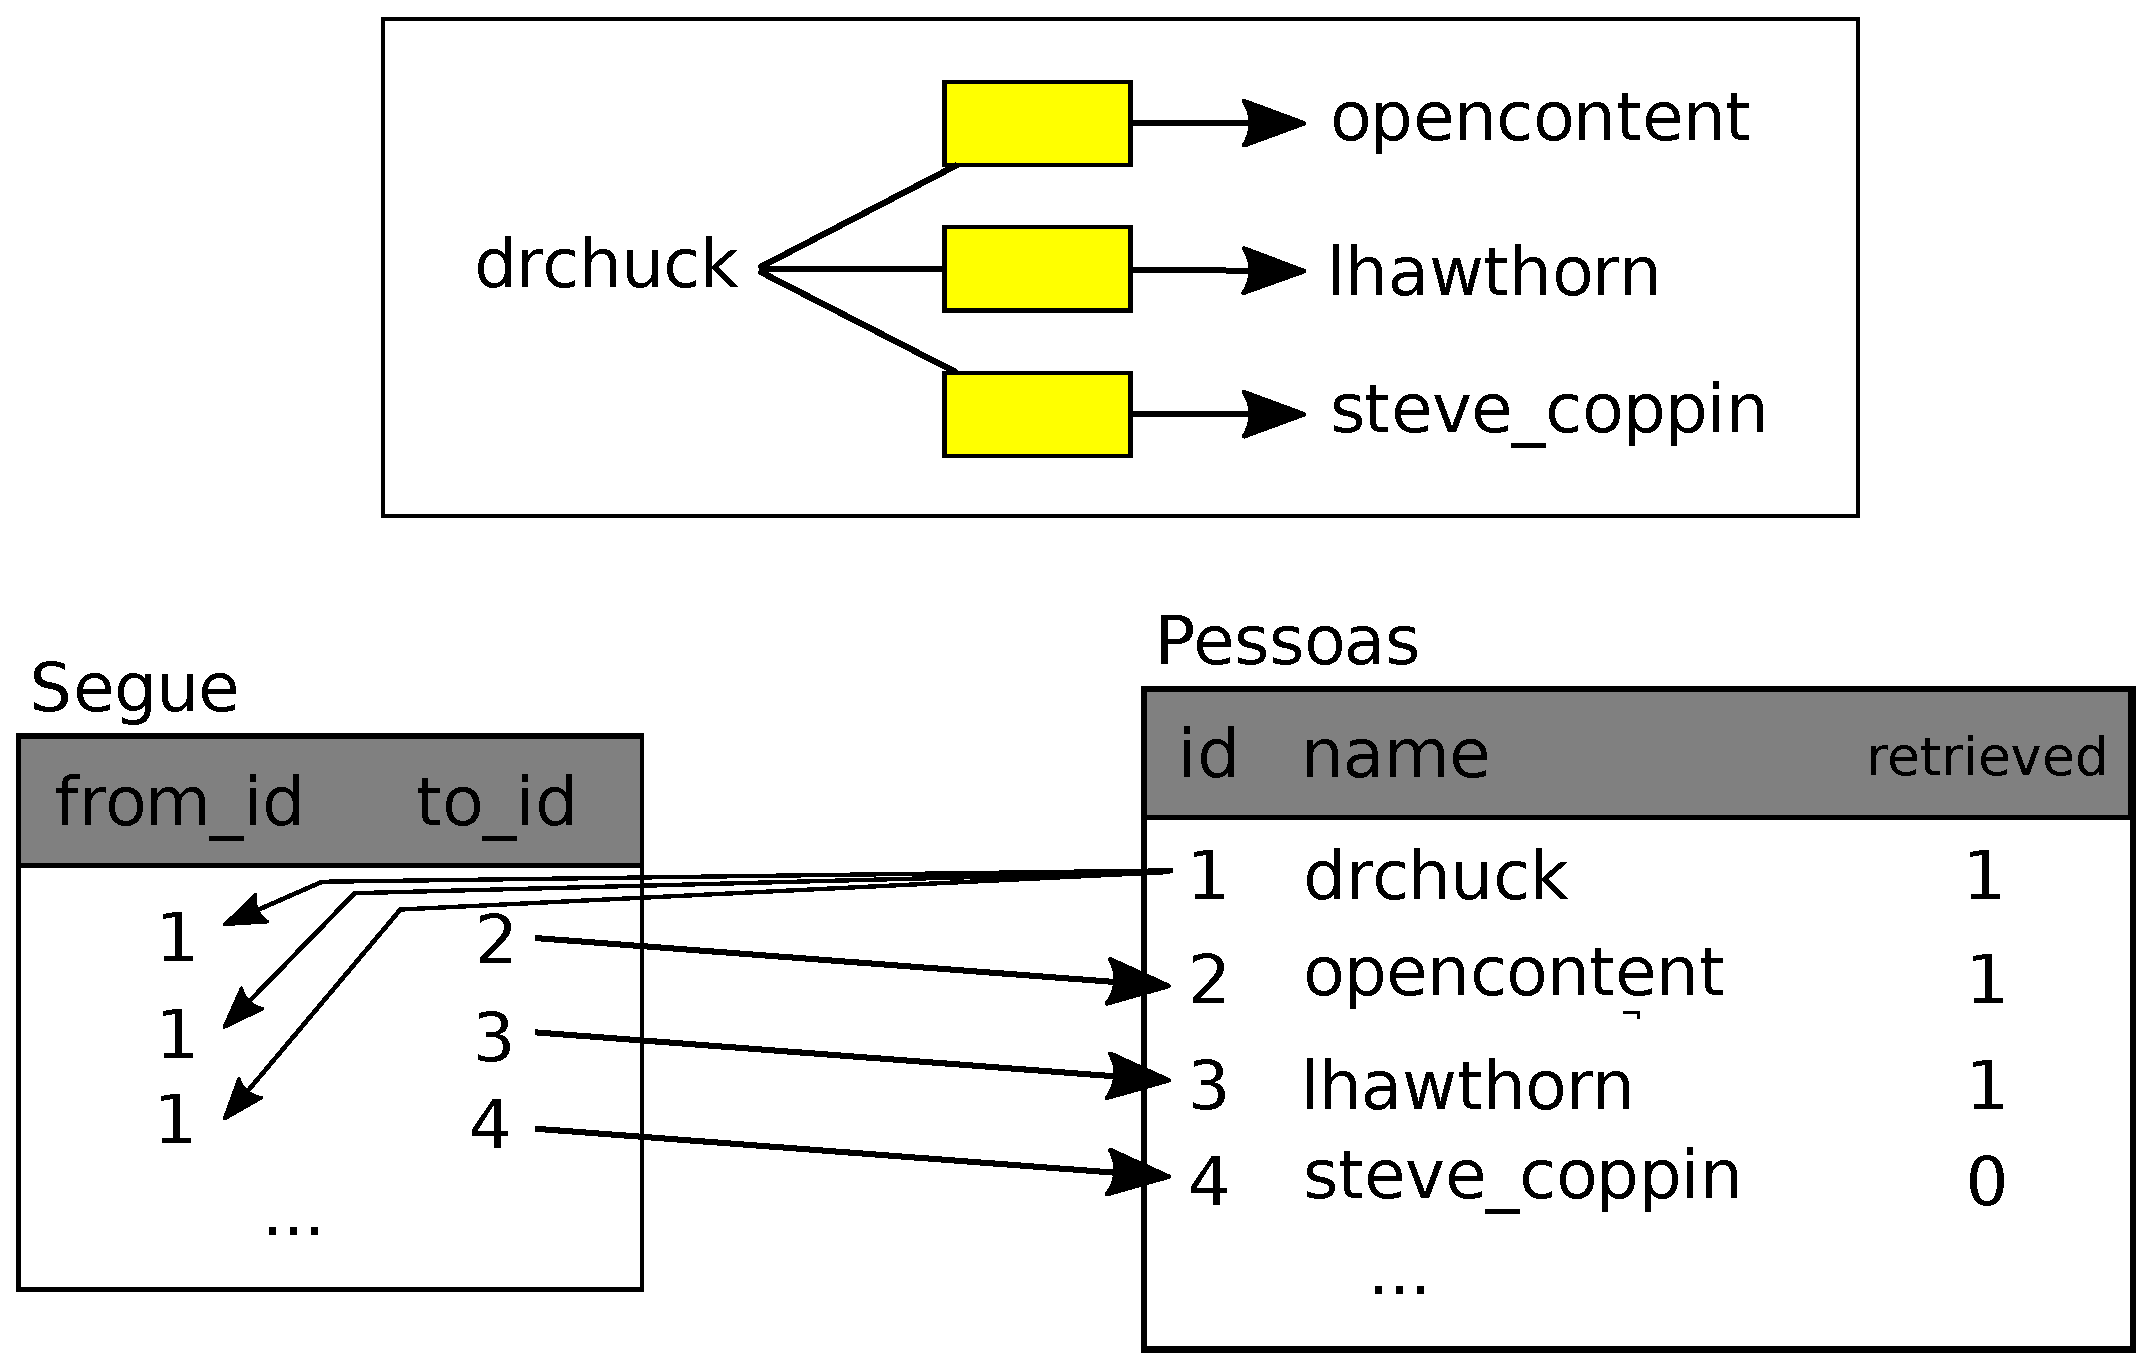
\includegraphics[height=2.50in]{figs2/twitter.eps}}
\afterfig


%\section{Programming with multiple tables}
\section{Programando com múltiplas tabelas}

%We will now redo the Twitter spider program using two tables, the primary
%keys, and the key references as described above.  Here is the code for 
%the new version of the program:

Agora nós iremos refazer o programa de rastreio do Twitter utilizando duas
tabelas, as chaves primárias, e as chaves de referências estão descritas
anteriormente. Abaixo está o código da nova versão do programa:

\beforeverb
\begin{verbatim}
import urllib
import twurl
import json
import sqlite3

TWITTER_URL = 'https://api.twitter.com/1.1/friends/list.json'

conn = sqlite3.connect('friends.sqlitesqlite3')
cur = conn.cursor()

cur.execute('''CREATE TABLE IF NOT EXISTS People 
    (id INTEGER PRIMARY KEY, name TEXT UNIQUE, retrieved INTEGER)''')
cur.execute('''CREATE TABLE IF NOT EXISTS Follows 
    (from_id INTEGER, to_id INTEGER, UNIQUE(from_id, to_id))''')

while True:
    acct = raw_input('Enter a Twitter account, or quit: ')
    if ( acct == 'quit' ) : break
    if ( len(acct) < 1 ) :
        cur.execute('''SELECT id, name FROM People 
            WHERE retrieved = 0 LIMIT 1''')
        try:
            (id, acct) = cur.fetchone()
        except:
            print 'No unretrieved Twitter accounts found'
            continue
    else:
        cur.execute('SELECT id FROM People WHERE name = ? LIMIT 1', 
            (acct, ) )
        try:
            id = cur.fetchone()[0]
        except:
            cur.execute('''INSERT OR IGNORE INTO People (name, retrieved) 
                VALUES ( ?, 0)''', ( acct, ) )
            conn.commit()
            if cur.rowcount != 1 : 
                print 'Error inserting account:',acct
                continue
            id = cur.lastrowid

    url = twurl.augment(TWITTER_URL, 
       {'screen_name': acct, 'count': '20'} )
    print 'Retrieving account', acct
    connection = urllib.urlopen(url)
    data = connection.read()
    headers = connection.info().dict
    print 'Remaining', headers['x-rate-limit-remaining']

    js = json.loads(data)
    # print json.dumps(js, indent=4)

    cur.execute('UPDATE People SET retrieved=1 WHERE name = ?', (acct, ) )

    countnew = 0
    countold = 0
    for u in js['users'] :
        friend = u['screen_name']
        print friend
        cur.execute('SELECT id FROM People WHERE name = ? LIMIT 1', 
            (friend, ) )
        try:
            friend_id = cur.fetchone()[0]
            countold = countold + 1
        except:
            cur.execute('''INSERT OR IGNORE INTO People (name, retrieved) 
                VALUES ( ?, 0)''', ( friend, ) )
            conn.commit()
            if cur.rowcount != 1 :
                print 'Error inserting account:',friend
                continue
            friend_id = cur.lastrowid
            countnew = countnew + 1
        cur.execute('''INSERT OR IGNORE INTO Follows (from_id, to_id) 
            VALUES (?, ?)''', (id, friend_id) )
    print 'New accounts=',countnew,' revisited=',countold
    conn.commit()

cur.close()
\end{verbatim}
\afterverb
%
%This program is starting to get a bit complicated, but it illustrates
%the patterns that we need to use when we are
%using integer keys to link tables. The basic patterns are:

%
Este programa está começando a ficar um pouco complicado, mas ilustra os
padrões que precisamos para utilizar quando estamos usando chaves inteiras
para conectar as tabelas. Os padrões básicos são:

\begin{enumerate}

%\item Create tables with primary keys and constraints.
\item Criar tabelas com chaves primárias e restrições.
%\item When we have a logical key for a person (i.e., account
%name) and we need the {\tt id} value for the person,
%depending on whether or not the person is already
%in the {\tt People} table we either need to: 
%(1) look up the person in the {\tt People} table and 
%retrieve the {\tt id} value for the person 
%or (2) add the person to the {\tt People} table and get the 
%{\tt id} value for the newly added row.
\item Quando temos uma chave lógica para uma pessoa (i.e., conta) e precisamos
  do valor de {\tt id} para a pessoa, dependendo se a pessoa já está na tabela
  {\tt People}  ou não, também precisaremos de: (1) olhar para a pessoa na
  tabela {\tt People} e recuperar o valor de {\tt id} da pessoa, ou (2)
  adicionar a pessoa na tabela {\tt People} e pegar o valor de {\tt id} para
  a nova linha recém adicionada.
  
%\item Insert the row that captures the ``follows'' relationship.

\item Inserir a linha que captura a relação com ``segue''.
  
\end{enumerate}

%We will cover each of these in turn.
Vamos tratar cada um dos ítens acima, em partes.

%\subsection{Constraints in database tables}
\subsection{Restrições em uma tabela}

As we design our table structures, we can tell the database system 
that we would like it to enforce a few rules on us.   These rules
help us from making mistakes and introducing incorrect data into 
out tables.   When we create our tables:
Assim como projetamos a estrutura da tabela, podemos informar ao banco de dados
que gostaríamos de reforçar algumas regras. Estas regras nos ajudam a não
cometer enganos e a não inserir dados incorretos nas nossas tabelas. Quando
criamos nossas tabelas:

\beforeverb
\begin{verbatim}
cur.execute('''CREATE TABLE IF NOT EXISTS People 
    (id INTEGER PRIMARY KEY, name TEXT UNIQUE, retrieved INTEGER)''')
cur.execute('''CREATE TABLE IF NOT EXISTS Follows 
    (from_id INTEGER, to_id INTEGER, UNIQUE(from_id, to_id))''')
\end{verbatim}
\afterverb
%
%We indicate that the {\tt name} column in the {\tt People} table must be
%{\tt UNIQUE}.   We also indicate that the combination of the two numbers
%in each row of the {\tt Follows} table must be unique.  These constraints
%keep us from making mistakes such as adding the same relationship more than
%once.
Indicamos que a coluna {\tt name} na tabela {\tt People} deve ser {\tt UNIQUE}.
Também indicaremos que a combinação dos dois números em cada linha da tabela
{\tt Follows} devem ser únicos. Estas restrições nos mantém longe da
possibilidade de cometer enganos como adicionar a mesma relação mais de uma vez.

%We can take advantage of these constraints in the following code:
Podemos obter vantagens destas restrições conforme mostra o seguinte código:

\beforeverb
\begin{verbatim}
cur.execute('''INSERT OR IGNORE INTO People (name, retrieved) 
    VALUES ( ?, 0)''', ( friend, ) )
\end{verbatim}
\afterverb
%
%We add the {\tt OR IGNORE} clause to our {\tt INSERT} statement to indicate
%that if this particular {\tt INSERT} would cause a violation of the
%``{\tt name} must be unique'' rule, the database system is allowed to ignore the 
%{\tt INSERT}.  We are using the database constraint as a safety net
%to make sure we don't inadvertently do something incorrect.
%
Adicionamos a condição {\tt OR IGNORE} a declaração {\tt INSERT} para indicar
que se este {\tt INSERT} em particular pode causar uma violação para a regra
``{\tt name} deve ser único'', assim o banco de dados tem permissão de ignorar
o {\tt INSERT}.

%Similarly, the following code ensures that we don't add the 
%exact same {\tt Follows} relationship twice.
De forma similar, o seguinte código garante que não adicionemos a mesma relação
{\tt Follows} duas vezes.

\beforeverb
\begin{verbatim}
cur.execute('''INSERT OR IGNORE INTO Follows 
    (from_id, to_id) VALUES (?, ?)''', (id, friend_id) )
\end{verbatim}
\afterverb
%
%Again, we simply tell the database to ignore our attempted 
%{\tt INSERT} if it would violate the uniqueness constraint
%that we specified for the {\tt Follows} rows.
Novamente, nós simplesmente dizemos para o banco de dados ignorar nossa
tentativa de inserir {\tt INSERT} se isto violar a regra de exclusividade que
especificamos para a linha {\tt Follows}.

%\subsection{Retrieve and/or insert a record}
\subsection{Restaurar e/ou inserir um registro}

%When we prompt the user for a Twitter account, if the account 
%exists, we must look up its {\tt id} value.  If the account
%does not yet exist in the {\tt People} table, we must insert 
%the record and get the {\tt id} value from the inserted
%row.

Quando solicitamos ao usuário uma conta do Twitter, se a conta existir,
precisamos verificar o valor do {\tt id}. Se a conta não existir ainda
na tabela {\tt People}, devemos inserir o registro e pegar o valor do
{\tt id} da linha inserida.

%This is a very common pattern and is done twice in the program above.
%This code shows how we look up the {\tt id} for a 
%friend's account when we have extracted a \verb"screen_name"
%from a {\tt user} node in the retrieved Twitter JSON.

Isto é um padrão muito comum e é feito duas vezes no programa acima. Este
código mostra como verificamos o {\tt id} da conta de um amigo, quando
extraímos um \verb"screen_name" de um nó de {\tt user} recuperado do JSON
do Twitter.

%Since over time it will be increasingly likely that the account
%will already be in the database, we first check to see if the
%{\tt People} record exists using a {\tt SELECT} statement.

Ao longo do tempo será cada vez mais provável que a conta já esteja registrada
no banco de dados, então primeiro checamos para ver se o registro existe em
{\tt People} utilizando uma declaração de {\tt SELECT}.

%If all goes well\footnote{In general, when a sentence starts 
%with ``if all goes well'' you will find that the code needs
%to use try/except.} inside the {\tt try} section, we retrieve the
%record using {\tt fetchone()} and then retrieve the
%first (and only) element of the returned tuple and store it in 
%\verb"friend_id".

Se tudo estiver certo\footnote{Em geral, quando uma sentença inicia com ``se
  tudo estiver certo'' você verá que o código precisa utilizar a condição
  {\it try/except}.} dentro da seção {\tt try}, recuperamos o registro usando
{\tt fetchone()} e depois recuperar o primeiro (e somente o primeiro) elemento
da tupla que retornou e a armazenamos em \verb"friend_id".

%If the {\tt SELECT} fails, the {\tt fetchone()[0]} code will fail
%and control will transfer into the {\tt except} section.

Se o {\tt SELECT} falhar, o código de {\tt fetchone()[0]} falhará e o controle
irá mudar para a seção {\tt except}.

\beforeverb
\begin{verbatim}
        friend = u['screen_name']
        cur.execute('SELECT id FROM People WHERE name = ? LIMIT 1',
            (friend, ) )
        try:
            friend_id = cur.fetchone()[0]
            countold = countold + 1
        except:
            cur.execute('''INSERT OR IGNORE INTO People (name, retrieved) 
                VALUES ( ?, 0)''', ( friend, ) )
            conn.commit()
            if cur.rowcount != 1 :
                print 'Error inserting account:',friend
                continue
            friend_id = cur.lastrowid
            countnew = countnew + 1
\end{verbatim}
\afterverb
%
%If we end up in the {\tt except} code, it simply means that the row
%was not found, so we must insert the row.  We use {\tt INSERT OR 
%IGNORE} just to avoid errors and then call {\tt commit()} to 
%force the database to really be updated.  After the write is done, we can 
%check the {\tt cur.rowcount} to see how many rows were affected.  Since
%we are attempting to insert a single row, if the number of 
%affected rows is something other than 1, it is an error.  

Se terminar no código do {\tt except}, isto significa que aquela linha não foi
encontrada, então devemos inserí-la na linha. Usamos o {\tt INSERT OR IGNORE}
somente para evitar erros e depois chamamos {\tt commit()} para forçar que a
base de dados seja atualizada. Depois que a escrita esteja completa, nós
podemos checar, com {\tt cur.rowcount}, para ver quantas linhas foram afetadas.
Uma vez que estamos tentando inserir uma simples linha, se o número de linhas
afetadas é alguma coisa diferente de 1, isto é um erro.

%If the {\tt INSERT} is successful, we can look at {\tt cur.lastrowid} 
%to find out what value the database assigned to the {\tt id} column in 
%our newly created row.

Se o {\tt INSERT} for executado com sucesso, nós podemos verificar, através do
{\tt cur.lastrowid} para descobrir qual valor o banco de dados associou na
coluna {\tt id} na nossa nova linha.

%\subsection{Storing the friend relationship}
\subsection{Armazenando a conexão do amigo}

%Once we know the key value for both the Twitter user
%and the friend in the JSON, it is a simple matter to insert
%the two numbers into the {\tt Follows} table
%with the following code:

Uma vez que sabemos o valor da chave para o usuário do Twitter e o amigo
extraído do JSON, simplesmente inserimos os dois números dentro da tabela
{\tt Follows} com o seguinte código:

\beforeverb
\begin{verbatim}
cur.execute('INSERT OR IGNORE INTO Follows (from_id, to_id) VALUES (?, ?)',
    (id, friend_id) )
\end{verbatim}
\afterverb
%
%Notice that we let the database take care of keeping us from ``double-inserting''
%a relationship by creating the table with a uniqueness constraint and then
%adding {\tt OR IGNORE} to our {\tt INSERT} statement.
%
Note que deixamos o banco de dados cuidar para nós de realizar a
``inserção-dupla'' da conexão criando a tabela com a restrição única e depois
adicionando {\tt OR IGNORE} a nossa condição de {\tt INSERT}.

%Here is a sample execution of this program:
Esta é um exemplo de execução deste programa:

\beforeverb
\begin{verbatim}
Enter a Twitter account, or quit: 
No unretrieved Twitter accounts found
Enter a Twitter account, or quit: drchuck
Retrieving http://api.twitter.com/1.1/friends ...
New accounts= 20  revisited= 0
Enter a Twitter account, or quit: 
Retrieving http://api.twitter.com/1.1/friends ...
New accounts= 17  revisited= 3
Enter a Twitter account, or quit: 
Retrieving http://api.twitter.com/1.1/friends ...
New accounts= 17  revisited= 3
Enter a Twitter account, or quit: quit
\end{verbatim}
\afterverb
%
%We started with the {\tt drchuck} account and then let the program
%automatically pick the next two accounts to retrieve and add to 
%our database.

%
Nós iniciamos com a conta {\tt drchuck} e depois deixamos o programa pegar
automaticamente as próximas duas contas para recuperar e adicionar a nossa
base de dados.

%The following is the first few rows in the {\tt People} 
%and {\tt Follows} tables after this run is completed:

Abaixo estão as primeiras linhas das tabelas {\tt People} e {\tt Follows}
depois que esta execução é finalizada:

\beforeverb
\begin{verbatim}
People:
(1, u'drchuck', 1)
(2, u'opencontent', 1)
(3, u'lhawthorn', 1)
(4, u'steve_coppin', 0)
(5, u'davidkocher', 0)
55 rows.
Follows:
(1, 2)
(1, 3)
(1, 4)
(1, 5)
(1, 6)
60 rows.
\end{verbatim}
\afterverb
%
%You can see the {\tt id}, {\tt name}, and {\tt visited} fields in the 
%{\tt People} table and you see the numbers of both ends of 
%the relationship in the {\tt Follows} table.   
%In the {\tt People} table, we can see that the first three people
%have been visited and their data has been retrieved.
%The data in the {\tt Follows} table indicates that
%{\tt drchuck} (user 1) is a friend to all of the people shown in the first
%five rows.  This makes sense because
%the first data we retrieved and stored was the Twitter friends of
%{\tt drchuck}.  If you were to print more rows from the {\tt Follows} table,
%you would see the friends of users 2 and 3 as well.

%
Você também pode ver os campos {\tt id}. {\tt name} e {\tt visited} na tabela
{\tt People} e os números dos finais das conexões na tabela {\tt Follows}. Na
tabela {\tt People}, podemos ver que as primeiras três pessoas foram visitadas
e seus dados foram recuperados. Os dados na tabela {\tt Follows} indica que
{\tt drchuck} (usuário 1) é amigo de todas as pessoas mostradas nas primeiras
cincos linhas. Isto mostra que o primeiro dado que recuperamos e armazenamos
foram dos amigos do {\tt drchuck}. Se você mostrou mais linhas da tabela
{\tt Follows}, você poderá ver os amigos dos usuários 2 e 3.

%\section{Three kinds of keys}
\section{Três tipos de chaves}

%Now that we have started building a data model putting our
%data into multiple linked tables and linking the rows in those
%tables using {\bf keys}, we need to look at some terminology 
%around keys.  There are generally three kinds of keys used 
%in a database model.

Agora que iniciamos a construção de um modelo de dados colocando nossos dados
dentro de múltiplas tabelas e linhas conectadas nestas tabelas utilizando
{\bf chaves}, precisamos olhar para algumas terminologias sobre as chaves.
Existem genericamentes três tipos de chaves que são utilizadas em um banco de
dados.

\begin{itemize}

%\item A {\bf logical key} is a key that the ``real world'' might use
%to look up a row.   In our example data model, the {\tt name}
%field is a logical key.  It is the screen name for the user 
%and we indeed look up a user's row several times in the program
%using the {\tt name} field.  You will often find that it makes
%sense to add a {\tt UNIQUE} constraint to a logical key.  Since the 
%logical key is how we look up a row from the outside world, it makes
%little sense to allow multiple rows with the same value in the table.

\item Um {\bf chave lógica} é uma chave que o ``mundo real'' pode usar para
  checar uma linha. Na nossa modelagem, o campo {\tt name} é uma chave lógica.
  Ele é o nome que usamos para o usuário e nós na verdade para uma linha de
  usuário diversas vezes no nosso programa usando o campo {\tt name}. Você
  perceberá que faz sentido adicionar a restrição de {\tt UNIQUE} para uma
  chave lógica. Uma vez que é através de chaves lógicas que consultamos uma
  linha do mundo exterior, faz um pouco de sentido permitir que múltiplas
  linhas tenham o mesmo valor em uma tabela.
  
%\item A {\bf primary key} is usually a number that is assigned
%automatically by the database.  It generally has no meaning outside
%the program and is only used to link rows from different tables
%together.  When we want to look up a row in a table, usually 
%searching for the row using the primary key is the fastest 
%way to find the row.  Since primary keys are integer numbers, they 
%take up very little storage and can be compared or sorted very quickly.
%In our data model, the {\tt id} field is an example of a primary key.

\item Um {\bf chave primária} é usualmente um número que é associado
  automaticamente por um banco de dados. Geralmente não terá significado fora
  do programa e só é utilizada para conectar as linhas de diferentes tabelas.
  Quando queremos verificar uma linha em uma tabela, normalmente buscamos pela
  linha utilizando a chave primária, é a forma mais rápida de encontrar uma
  linha. Uma vez que chaves primárias são números inteiros, eles ocupam pouco
  espaço e podem ser comparados ou ordenados rapidamente. No nosso modelo, o
  campo {\tt id} é um exemplo de chave primária.
  
%\item A {\bf foreign key} is usually a number that points to the primary key
%of an associated row in a different table.  An example of a foreign
%key in our data model is the \verb"from_id".  

\item Uma {\bf chave estrangeira} é normalmente um número que aponta para a
  chave primária associada a uma linha em outra tabela. Um exemplo de chave
  estrangeira no nosso modelo é o campo \verb"from_id".
\end{itemize}

%We are using a
%naming convention of always calling the primary key field name
%{\tt id} and appending the suffix \verb"_id" to any field name
%that is a foreign key.

Nós estamos utilizando uma convenção de sempre chamar uma chave primária de
um campo {\tt id} e adicionando o sufixo \verb"_id" para qualquer campo que
seja uma chave estrangeira.

%\section{Using JOIN to retrieve data}
\section{Utilizando o JOIN para recuperar informações}

%Now that we have followed the rules of database normalization
%and have data separated into two tables, linked together using
%primary and foreign keys, we need to be able to build a 
%{\tt SELECT} that reassembles the data across the tables.

Agora que seguimos as regras de normalização de bancos de dados e temos os
dados separados em duas tabelas, associadas através de chaves primárias e
chaves estrangeiras, precisamos ser capazes de construir uma chamada de
{\tt SELECT} que reagrupa os dados em toda as tabelas.

%SQL uses the {\tt JOIN} clause to reconnect these tables.  
%In the {\tt JOIN} clause you specify the fields that are used 
%to reconnect the rows between the tables.

SQL utiliza a cláusula {\tt JOIN} para reconectar estas tabelas. Na cláusula
{\tt JOIN} você especifica o campo que serão utilizados para reconectar as
linhas entre as tabelas.

%The following is an example of a {\tt SELECT} with a 
%{\tt JOIN} clause:

Abaixo, um exemplo de um {\tt SELECT} com um {\tt JOIN}:

\beforeverb
\begin{verbatim}
SELECT * FROM Follows JOIN People 
    ON Follows.from_id = People.id WHERE People.id = 1
\end{verbatim}
\afterverb
%
The {\tt JOIN} clause indicates that the fields we are selecting
cross both the {\tt Follows} and {\tt People} tables.  The {\tt ON}
clause indicates how the two tables are to be joined:  Take the rows
from {\tt Follows} and append the row from {\tt People} where the
field \verb"from_id" in {\tt Follows} is the same the {\tt id} value
in the {\tt People} table.

%
O {\tt JOIN} indica que o cmapo que utilizamos são selecionados cruzando ambas
as tabelas {\tt Follows} e {\tt People}. A cláusula {\tt ON} indica como as
duas tabelas devem ser unidas: Junta as linhas da tabela {\tt Follows} às da
tabela {\tt People} onde o campo \verb"from_id" em {\tt Follows} tem o mesmo
valor do campo {\tt id} na tabela {\tt People}.

\beforefig
\centerline{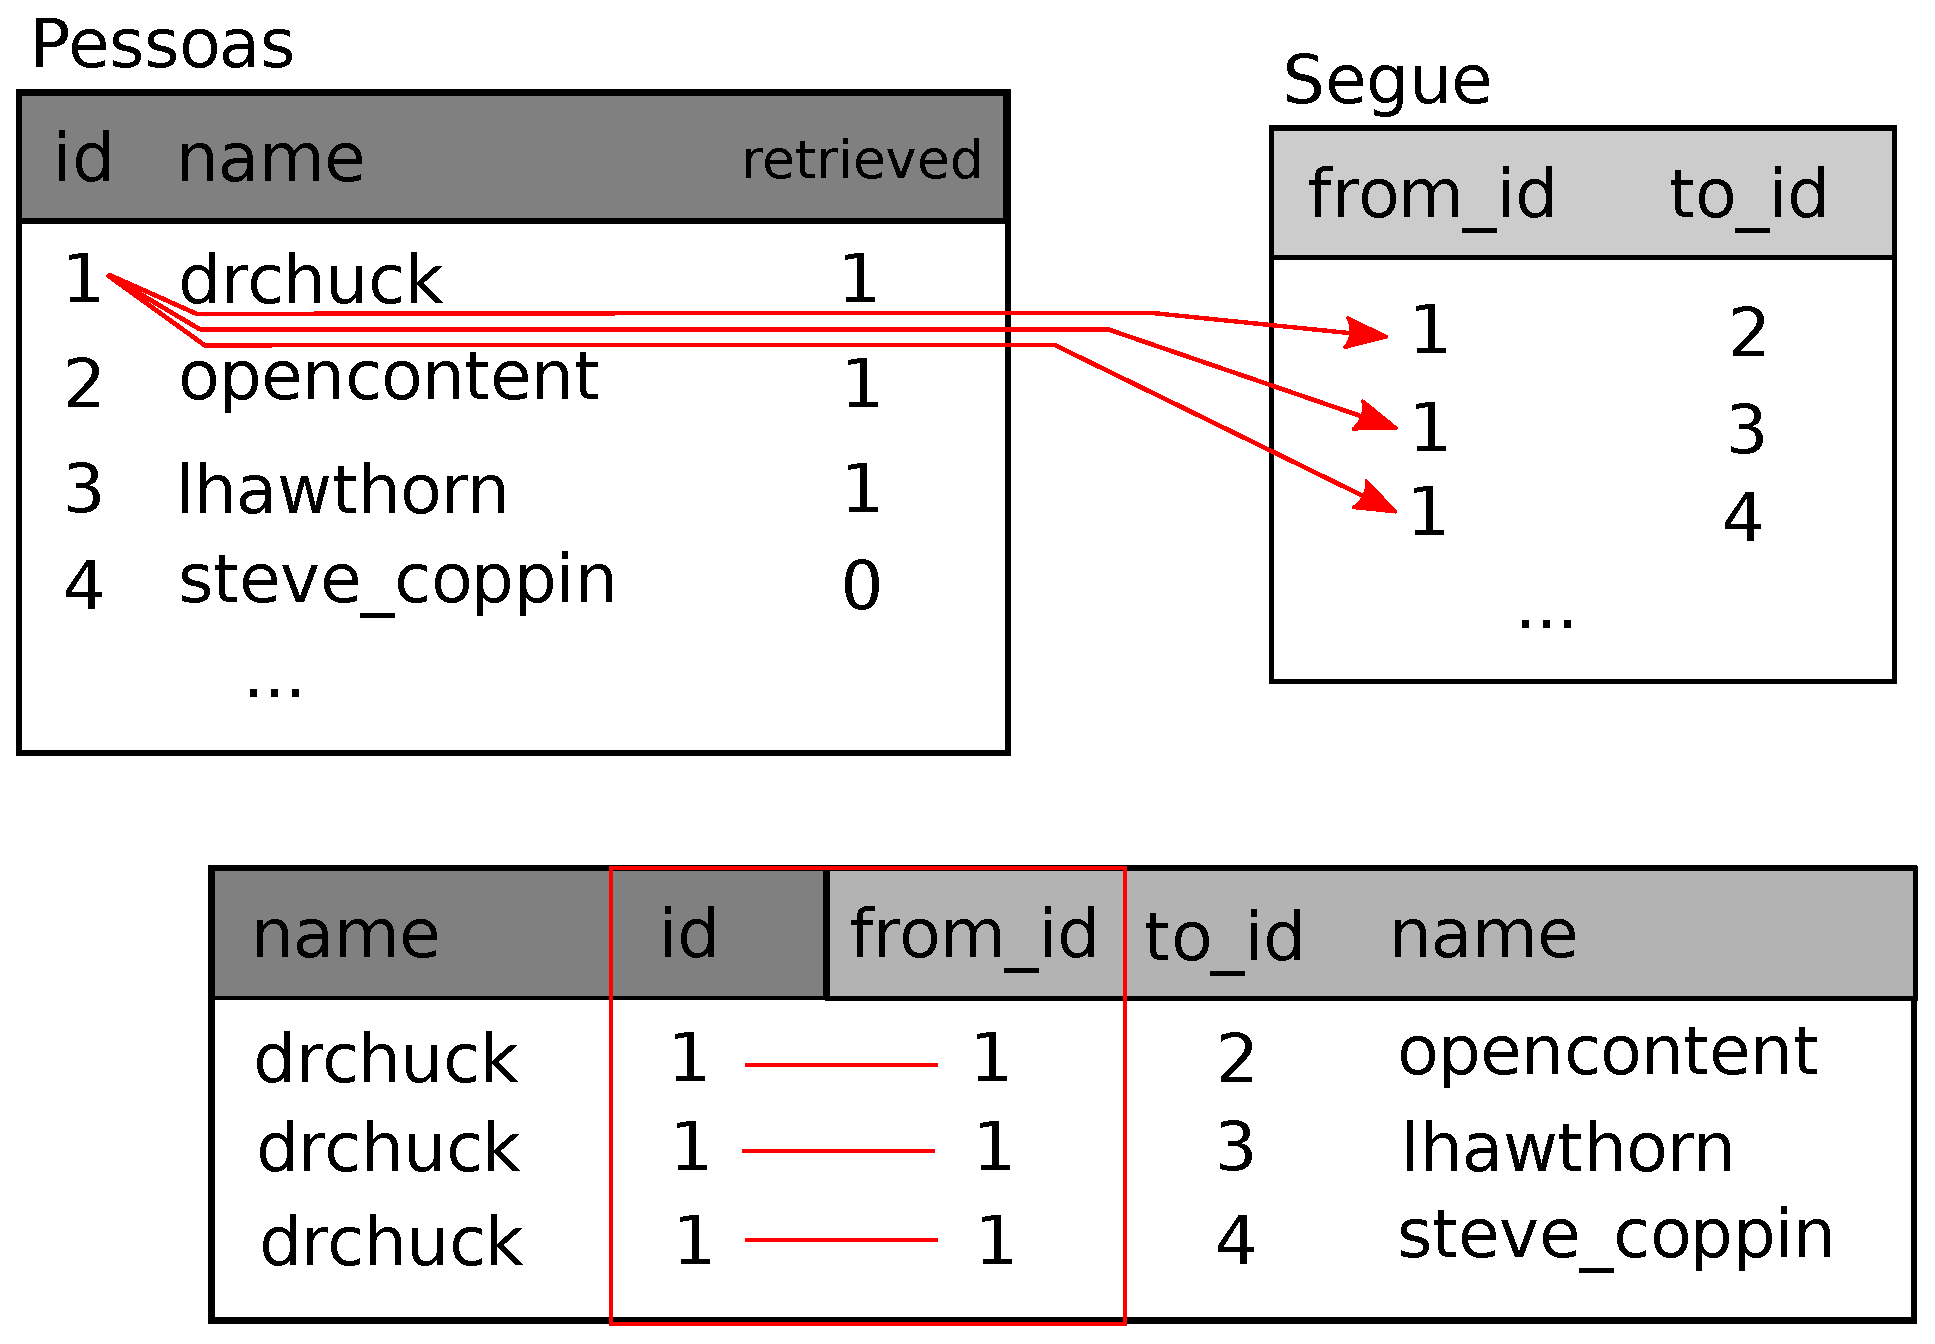
\includegraphics[height=2.50in]{figs2/join.eps}}
\afterfig

%The result of the JOIN is to create extra-long ``metarows'' which have both 
%the fields from {\tt People} and the matching fields from {\tt Follows}.
%Where there is more than one match between the {\tt id} field from {\tt People}
%and the \verb"from_id" from {\tt People}, then JOIN creates a metarow 
%for \emph{each} of the matching pairs of rows, duplicating data as needed.

O resultado do {\tt JOIN} cria uma super ``metalinha'' que tem os dois campos
da tabela {\tt People} que casam com os campos da tabela {\tt Follows}. Onde
existir mais de uma ocorrência entre o campo {\tt id} e o \verb"from_id" da
tabela {\tt People}, então o {\tt JOIN} cria uma ``metalinha'' para \emph{cada}
par de linhas que correspondem, duplicando os dados conforme for necessário.

%The following code demonstrates the data that we will have in the 
%database after the multi-table Twitter spider program (above) has
%been run several times.

O seguinte código demonstra o dado que nós teremos no banco de dados após o
executar o programa coletor de dados (acima) diversas vezes.

\beforeverb
\begin{verbatim}
import sqlite3

conn = sqlite3.connect('spider.sqlite3')
cur = conn.cursor()

cur.execute('SELECT * FROM People')
count = 0
print 'People:'
for row in cur :
   if count < 5: print row
   count = count + 1
print count, 'rows.'

cur.execute('SELECT * FROM Follows')
count = 0
print 'Follows:'
for row in cur :
   if count < 5: print row
   count = count + 1
print count, 'rows.'

cur.execute('''SELECT * FROM Follows JOIN People 
    ON Follows.to_id = People.id WHERE Follows.from_id = 2''')
count = 0
print 'Connections for id=2:'
for row in cur :
   if count < 5: print row
   count = count + 1
print count, 'rows.'

cur.close()
\end{verbatim}
\afterverb
%
%In this program, we first dump out the {\tt People}
%and {\tt Follows} and then dump out a subset of the
%data in the tables joined together.

%
Neste programa, primeiro descarregamos a tabela {\tt People} e {\tt Follows} e
depois descarregamos um subconjunto de dados das tabelas juntos.

%Here is the output of the program:

Aqui temos a saída do programa:

\beforeverb
\begin{verbatim}
python twjoin.py 
People:
(1, u'drchuck', 1)
(2, u'opencontent', 1)
(3, u'lhawthorn', 1)
(4, u'steve_coppin', 0)
(5, u'davidkocher', 0)
55 rows.
Follows:
(1, 2)
(1, 3)
(1, 4)
(1, 5)
(1, 6)
60 rows.
Connections for id=2:
(2, 1, 1, u'drchuck', 1)
(2, 28, 28, u'cnxorg', 0)
(2, 30, 30, u'kthanos', 0)
(2, 102, 102, u'SomethingGirl', 0)
(2, 103, 103, u'ja_Pac', 0)
20 rows.
\end{verbatim}
\afterverb
%
%You see the columns from the {\tt People} and {\tt Follows} tables and the last
%set of rows is the result of the {\tt SELECT} with the {\tt JOIN} clause.

%
Você vê as colunas das tabelas {\tt People} e {\tt Follows} e por último
conjunto de linhas é o resultado do {\tt SELECT} com o {\tt JOIN}.

%In the last select, we are looking for accounts that are friends of 
%``opencontent'' (i.e., {\tt People.id=2}).

No último {\tt SELECT}, nós estamos procurando por contas que tem amigos de
``conteúdo aberto'' (i.e., {\tt People.id=2}).

%In each of the ``metarows'' in the last select, the first two columns are
%from the {\tt Follows}
%table followed by columns three through five from the {\tt People} table.  You can also
%see that the second column (\verb"Follows.to_id") matches the third column
%({\tt People.id}) in each of the joined-up ``metarows''.


Em cada uma das ``meta-linhas'' da última seleção, as primeiras duas colunas
são da tabela {\tt Follows} seguidas pelas colunas três até cinco da tabela
{\tt People}. Você também pode ver que a segunda coluna (\verb"Follows.to_id")
relaciona a terceira coluna ({\tt People.id}) em cada uma das ``meta-linha''
que foram juntas.

%\section{Summary}
\section{Sumário}

%This chapter has covered a lot of ground to give you an overview of the basics
%of using a database in Python.   It is more complicated to write the code to use 
%a database to store data than Python dictionaries or flat files so there is 
%little reason to use a database unless your application truly needs the capabilities
%of a database.  The situations where a database can be quite useful are: 
%(1) when your application needs to make small many random updates within a large data set,
%(2) when your data is so large it cannot fit in a dictionary and you need to 
%look up information repeatedly, or (3) when you have a long-running process that you
%want to be able to stop and restart and retain the data from one run to the next.

Este capítulo cobriu os fundamentos para o uso, básico, de banco de dados no
Python. É muito mais complicado escrever código para usar um banco de dados
para armazenar informações do que dicionários ou arquivos com Python, então
se existe poucas razões para utilizar um banco de dados, a menos que sua
aplicação realmente precise das capacidades de um banco de dados. As situações
onde um banco de dados podem ser muito úteis são: (1) quando sua aplicação
precisa realizar pequenas atualizações com um conjunto grande de dados, (2)
quando seus dados são tão grandes que não podem ser armazenados em um
dicionário e você precisa acessar estas informações repetidas vezes, ou (3)
quando você tem um processo de execução demorada e você quer ser capaz de
parar e recomeçar e manter os dados entre as pesquisas.

%You can build a simple database with a single table to suit many application 
%needs, but most problems will require several tables and links/relationships
%between rows in different tables.   When you start making links between 
%tables, it is important to do some thoughtful design and follow the 
%rules of database normalization to make the best use of the database's
%capabilities.  Since the primary motivation for using a database
%is that you have a large amount of data to deal with, it is important
%to model your data efficiently so your programs run as fast as possible.

Você pode construir um banco de dados simples com uma única tabela para
atender muitas aplicações, mas a maiorias dos problemas vão necessitar de
várias tabelas e conexões/relações entre as linhas em diferentes tabelas.
Quando você começar a fazer relações entre as tabelas, é importante fazer
algum planejamento e seguir as regras de normatização de banco de dados
para fazer um melhor uso das capacidades dos bancos de dados. Uma vez que a
principal motivação para utilizar um banco de dados é que você tem um grande
conjunto de dados para tratar, é importante modelar os dados eficientemente,
assim seus programas poderão rodas tão rápido quanto for possível.

%\section{Debugging}
\section{Depuração}
%One common pattern when you are developing a Python program to connect to
%an SQLite database will be to run a Python program and check the
%results using the SQLite Database Browser.  The browser allows you 
%to quickly check to see if your program is working properly.

É comum quando você está desenvolvendo um programa em Python para se conectar
em um banco de dados SQLite, é executar um programa para checar os resultados
utilizando o Navegador SQLite. O navegador permitirá que rapidamente verifique
se o seu programa está funcionando corretamente.

%You must be careful because SQLite takes care to keep two programs
%from changing the same data at the same time.   For example, if
%you open a database in the browser and make a change to the database
%and have not yet pressed the ``save'' button in the browser, the 
%browser ``locks'' the database file and keeps any other program
%from accessing the file.  In particular, your Python program
%will not be able to access the file if it is locked.

Você deve ter cuidado, porque o SQLite cuida para que dois programas não
façam modificações nos dados ao mesmo tempo. Por exemplo, se você abrir
um banco de dados no navegador e faz alterações no banco de dados, enquanto
não pressionar o botão ``salvar'', o navegador ``trava'' o arquivo do banco
de dados e impede qualquer outro programa de acessar o arquivo. Desta forma
seu programa em Python não conseguirá acessar o arquivo se ele estiver travado.

%So a solution is to make sure to either close the database browser 
%or use the {\bf File} menu to close the database in the browser
%before you attempt to access the database from Python to avoid
%the problem of your Python code failing because the database is
%locked.

Então, uma solução é garantir que fechou o navegador ou utilizar o menu
{\bf Arquivo} para fechar o banco de dados no navegador antes de tentar
acessar o banco de dados através do Python, evitando problemas no seu código
porque o banco de dados está travado.

%\section{Glossary}
\section{Glossário}

\begin{description}


%\item[attribute:] One of the values within a tuple.  More commonly
%called a ``column'' or ``field''.
%\index{attribute}

\item[atributo:] Um dos valores dentro de uma tupla. Comumente chamado de
  ``coluna'' ou ``campo''.
  \index{atributo}
  
%\item[constraint:] 
%When we tell the database to enforce a rule on a field or a row
%in a table.  A common constraint is to insist that there can be no
%duplicate values in a particular field (i.e., all the values must be unique).
  %\index{constraint}
  
\item[restrição:] Quando ordenamos a um banco de dados para reforçar uma regra
em um campo ou em uma linha na tabela. Uma restrição comum é insistir que não
pode haver valore duplicados em um campo em particular (i.e., todos os
valores tem que ser únicos).
\index{restrição}


%\item[cursor:] A cursor allows you to execute SQL commands in a database
%and retrieve data from the database.  A cursor is similar to 
%a socket or file handle for network connections and files, respectively.
%\index{cursor}

\item[cursor:] Um cursor permite execução de um comando SQL em um banco de
  dados e recuperar informações de um banco de dados. Um cursor é similar a
  um {\it socket} ou identificador de arquivos para uma conexão de rede e
  arquivos, respectivamente.
  \index{cursor}
  
%\item[database browser:] 
%A piece of software that allows you to directly connect to a database 
%and manipulate the database directly without writing a program.
%\index{database browser}

\item[navegador de banco de dados:] um conjunto de {\it software} que permite
  se conectar diretamente a um banco de dados e manipulá-lo diretamente, sem
  escrever um programa.
  \index{navegador de banco de dados}
  
%\item[foreign key:] A numeric key that points to the primary key of 
%a row in another table.  Foreign keys establish relationships between rows
%stored in different tables.
%\index{foreign key}

\item[chave estrangeira:] Uma chave numérica que aponta para uma chave primária
  de uma linha em outra tabela. Chaves estrangeiras estabelecem relações entre
  linhas armazenadas em diferentes tabelas.
  \index{chave estrangeira}
  
%\item[index:] Additional data that the database software maintains as rows
%and inserts into a table to make lookups very fast.
%\index{index}

\item[índice:] Dados adicionais que um banco de dados mantém, como linhas e
  inserções dentro de uma tabela para realizar consultas mais rápido.
  \index{índice}
  
%\item[logical key:] A key that the ``outside world'' uses to look up a particular
%row.  For example in a table of user accounts, a person's email address
%might be a good candidate as the logical key for the user's data. 
%\index{logical key}

\item[chave lógica:] Uma chave que o ``mundo externo'' utiliza para consultar
  uma linha em particular. Por exemplo em uma tabela de contas de usuários, o
  email de uma pessoa pode ser um bom candidato a chave lógica para a
  informação de usuário.
  \index{chave lógica}
  
%\item[normalization:] Designing a data model so that no data
%is replicated.  We store each item of data at one place in the database
%and reference it elsewhere using a foreign key.
%\index{normalization}
%\index{database normalization}

\item[normatização:] Projetar um modelo de dados para que nenhum dado seja
  replicado. Armazenamos cada item de dados em um lugar no banco de dados
  e referenciamos isso em qualquer lugar utilizando chave estrangeira.
  \index{normatização}
  \index{normatização de banco de dados}
  
%\item[primary key:] A numeric key assigned to each row that is used to 
%refer to one row in a table from another table.  Often the database
%is configured to automatically assign primary keys as rows are inserted.
%\index{primary key}

\item[chave primária:] Uma chave numérica associada a cada linha que é usada
  para referenciar uma linha em uma tabela de outra tabela. Normalmente o
  banco de dados é configurado para automaticamente associar chaves primárias
  assim que linhas são inseridas.
  \index{chave primária}
  
%\item[relation:] An area within a database that contains tuples and 
%attributes.  More typically called a ``table''.
%\index{relation}

\item[relação:] Uma área dentro do banco de dados que contém tuplas e
  atributos. Tipicamente chamada de ``tabela''.
  \index{relação}
  
%\item[tuple:] A single entry in a database table that is a set 
%of attributes.  More typically called ``row''.
%\index{tuple}

\item[tupla:] Uma entrada em um banco de dados que é um conjunto de atributos.
  Tipicamente chamado de ``linha''.
  \index{tupla}
\end{description}

